Article: Improving CUSUM performance in presence of prediction intervals

\begin{abstract}
In the real world, the data tends to change over time.
Machine learning systems need to have mechanisms for monitoring changes in data distributions, for continuous diagnostics of their models performance, and for model adaptations that can handle concept drifts, i.e.\ sudden or gradual changes in underlying data distributions.
The so-called informed methods for handling concept drift are based on online change detection mechanisms. Most of the existing mechanisms assume that changes are not predictable.
However, there are various application settings in which concept drifts are expected to reoccur with a pattern.
Intuitively, contextual information about past and future change points locations may help to perform online change detection with shorter delays and with lower false alarm rates.
We show how this performance gain can be achieved for Cusum detector as one of the most popular detection methods based on sequential analysis, in presence of prediction intervals capturing change points locations.
% We study the settings when the prior information about when changes are likely to happen is available.
% We show the potential and limitation of using such prior information when it is available as a background knowledge.
% No: We explore the relation of optimal settings of dynamic and static detectors on both synthetic and real word datasets and provide guidelines how to use the prior information for online change detection in practice.
% Done in previous work: We demonstrate how we can learn such priors from the data as a predictive confidence change function and how we can use it with CUSUM detector to adjust its sensitivity dynamically.
% Intuitively, using some form of recurrence or external contextual information may help to perform online change detection with shorter delays and with lower false alarm rates.
%\keywords{Change detection \and Concept drift \and Cusum \and Prediction}
\end{abstract}


\section{Introduction}~\label{sec:intro}
% https://www.itl.nist.gov/div898/handbook/mpc/section2/mpc21.htm
Machine learning under concept drift has been an actively studied research area. \cite{gama2014survey} and \cite{zliobaite2016overview} provide comprehensive overviews of methods and studied application scenarios. As the data distributions change over time, machine learning models need to adapt to these changes in a timely manner. The so-called informed adaptation methods rely on on-line change detectors that trigger an adaptation mechanism. 

% The problem of on-line change detection in time series is closely related to the concept drift problem~\cite{zliobaite2010learning,gama2014survey,zliobaite2016overview,tsymbal2004problem} in Machine Learning area. Concept drift is a change in the underlying data distribution (concept), from which machine learning model was induced~\cite{SouzaRMB20}, resulting in the degraded model performance. The issue becomes critical once model retraining becomes expensive with the growing volume of new input data instances arriving continuously as a stream. The first step to deal with the issue is to detect model performance degradation as soon as possible in order to take action to fix it. This can be done by applying change detection methods to model performance metrics observed over time.
%Time series depicts temporal evolution of a process or phenomenon.
%The underlying system or data generation mechanism may change its behaviour between different phases of the process.The problem of on-line change detection is faced in many application domains in science, medicine, and engineering.
On-line change detection in time series data is an old practical problem with the roots in the problem of statistical quality control~\cite{basseville1993detection}, ~\cite{NISTbook}.
Walter A. Shewhart invented control charts in 1924 while working on the problem of statistical quality control to improve reliability of telephone transmission systems.
% > https://www.itl.nist.gov/div898/handbook/pmc/section1/pmc11.htm
% > The first to apply the newly discovered statistical methods to the problem of
% > quality control was Walter A. Shewhart of the Bell Telephone Laboratories. He
% > issued a memorandum on May 16, 1924 that featured a sketch of a modern control
% > chart.
%In 1931 he summarized his ideas in the classical book ``Economic Control of Quality Of Manufactured Product''~\cite{shewhart1931economic}.
%Basically a production process can be in-control, or in out-of-control state.
%If the process is out of control, then the quick and reliable detection of such a state can maximize cost savings.
%quickest detection with as low as possible false alarm (FA) rate is the best solution for minimizing production costs.
%TOMMI: Check the last part of next sentence: could ARL really be the same as expected number of observations before detection?
Commonly used change detection performance metrics are the mean detection delay and mean time between false alarms which is also referred as average run length (ARL), which is an expected number of observations before detection is alarmed~\cite{basseville1993detection}.
When designing a change detector the goal is to find an optimal trade off between these metrics by adjusting detector's sensitivity.
Once adjusted, the detector is %usually further
then further used with the obtained optimal settings.
We refer to this type of detector as a \textit{static settings detector}, i.e.,\ detector with fixed, static settings.
%We address to the following research questions.
But what if we know that the next change is most likely to appear within a given time interval in the future?
With such a recurring nature of change points, we could
%Then we can
disregard %all detections outside this interval
improbable detections not following the statistics of change point recurrency.
%and collect all detections within it.
In this way, we would decrease the number of false alarm (FA) events while keeping detection delay on a desirable level.
We refer this type of a detector as a \textit{dynamic settings detector}.
First research question related to such a detector is how to predict the time intervals assuming that changes recur and what are the confidence intervals for those predictions?
Moreover, once the number of FA events is decreased, the question is\ -\ can we decrease the detection delay further by increasing the sensitivity of the dynamic detector?

For estimating the change point prediction intervals used by the dynamic detector, we use the Predictive confidence change function (Pccf) introduced in our previous work~\cite{MaslovSDM2016}. 
We show that using prediction intervals the CuSum change detection performance can be improved compared to the static settings if the ARL corresponding to the dynamic threshold value is smaller than the width of prediction interval.
Also, as long as the prediction interval encapsulates the change locations, the FA rate can be decreased safely by just ignoring detections outside the prediction interval.
Reduction of the detection delay in dynamic settings is not guaranteed, since the probability of FA increases proportionally to the detector's level of sensitivity.
However, we expect that the likelihood of FA within relatively narrow prediction intervals will still be lower than across whole signal allowing detection with a smaller delay and a lower FA rate.
%  % Sec.3.1.4.1
%  Brownian motion can be seen as the limit of cumulative sums of independent, identically distributed random  variables. A precise statement of this limiting property in terms of a representation and a convergence  theorem for cumulative sums can be found in [Breiman, 1968, Billingsley, 1968]. Because of this, Brownian  motion is of key interest in this book because of the central role played by sequential hypotheses testing and  Cusum algorithm for change detection. Moreover, Brownian motion can be seen as the limit of some  martingales [P.Hall and Heyde, 1980].
%
%The proposed dynamic approach is composed of two main steps.
%In the first step, we apply the Pccf to predict the time intervals where changes are most likely to occur. 
%In the second step, we then detect changes using dynamically adjusted change detector.
To confirm reduction both in FA rate and in detection delay when using prediction intervals we conduct experiments with simulated data and with a real signal with known ground truth change points and their locations. 
%Our experimental result show that despite increasing probability of false alarm events when increasing sensitivity within prediction intervals with shorter delay because likelihood of FA within relatively narrow prediction intervals will still be lower than across whole signal allowing detection with a smaller delay and a lower FA rate.
Our empirical results are further explained using the random walk property of the 
CuSum output statistic~\cite{billingsley2013convergence, basseville1993detection,veeravalli2014quickest}.

The current work continues our earlier efforts in the research field.
In~\cite{MaslovSDM2016} we developed a predictive confidence change function (Pccf) to calculate prediction intervals for recurrent change points.
In~\cite{MaslovIJCNN2017} we developed a Bayesian learn predict adjust method (BLPA) where Pccf is used in Bayesian settings under various uncertainty assumptions and performance is measured by considering maximum allowed detection delay, so that all detections alarmed within maximum allowed delay after changepoint are considered equally successful no matter of delay values. 
Novel contributions in this work are
\begin{enumerate}
    \item In experiments we demonstrate that given prediction intervals capturing change points locations the detection delay can be decreased by lowering detection threshold $h$ value within prediction intervals without increasing false alarm rate.  
    
    \item We explain why detection delay is decreased without increased FA rate using a random walk property of the CuSum output statistic and by using the property that ARL value decreases proportionally to the threshold $h$. ARL corresponding to the threshold $h$ should not be larger than the width of the prediction interval, otherwise detection will happen outside ROI\footnote{This issue can be potentially resolved by using a backtracking mechanism to locate change point in the past, but this is out of scope of the current work}.
    
    \item As a minor improvement, we describe a more concise way of calculating Pccf than in the previous work, and we calculate Pccf for several commonly used for inter-arrival times modelling distributions.

\end{enumerate}
Implementation and data used in the experiments are shared as a Python package~\footnote{\href{https://github.com/av-maslov/pccf}{https://github.com/av-maslov/pccf}}.
%\item In experiments we demonstrate that given prediction intervals capturing change points locations a) false alarm rate can be reduced by ignoring detections outside prediction intervals, at the least, and, as a second step,- b) the detection delay can be decreased by lowering detection threshold $h$ value within prediction intervals.
%\item In experiments we demonstrate the counter-intuitive result that despite increasing probability of false alarm events due to the decreased threshold value $h$, performance both in terms of the detection delays and smaller FA rate can be achieved. This is possible due to the simple reason that length of prediction intervals is smaller than length of the input signal.

The paper is organised as follows.
In the Section~\ref{sec:cusum_detector} we describe CuSum detector and its statistical properties important both for defining performance metrics and for theoretical understanding why and how performance can be improved in dynamic settings.
In the Section~\ref{sec:pccf} we outline Pccf calculation used to forecast prediction intervals for change points.
In the Section~\ref{sec:performance} we define change detection performance metrics to be used in Experiments section.
In the Section~\ref{sec:experiments} we perform experimental study with artificially generated time series and with temperature measurements collected from the sensor installed in the home office environment.
Finally, based on obtained results we make conclusions and outline limitations of the proposed framework in the section~\ref{sec:conclusions}.


\section{Related work}~\label{sec:related_work}
Many change detectors for univariate and multivariate data have been introduced in the literature. They can be used to monitor changes in feature distributions or changes in accuracy of predictors. Three main categories of change detectors can be considered: methods based on detecting differences between two distributions using e.g.\ Kullback–Leibler divergence or Kolmogorov–Smirnov test, methods based on statistical process control, e.g.\ tracking number of error classifications as in DDM~\cite{gama2004learning} or number of examples between classification errors as in EDDM~\cite{baena2006early}, and methods based on sequential analysis, e.g.\ Sequential Probability Ratio Test used in CuSum and Page–Hinkley~\cite{Page1954} and and Bayesian based approaches, e.g.~\cite{girshick1952bayes}. 

In this work we use CuSum control charts~\cite{Page1954} because of it simplicity and transparent statistical properties.
We address the problem of reducing detection delay using prediction intervals. 
The problem related to the optimality of change detection procedure.
% % https://arxiv.org/pdf/1210.5552.pdf
Optimality of the change detection procedure was investigated in~\cite{Page1954},~\cite{Shiryaev2010,Shiryaev1961,Shiryaev1963}.
Asymptotic and nonasymptotic optimality of cumulative sum algorithms was proved in~\cite{lorden1971procedures},~\cite{moustakides1986optimal},~\cite{moustakides2004optimality},~\cite{ritov1990decision}.
In~\cite{Shiryaev1963,shiryaev2007optimal} the change point is modelled as a random variable with a known geometric distribution~\cite{veeravalli2014quickest} and optimal algorithm minimizing the average detection delay given constraint on the probability of false alarm is proposed. In our work we minimize the detection delay given a constraint on the maximum delay imposed by the prediction interval width. In~\cite{lorden1971procedures} asymptotic optimality of Cusum~\cite{Page1954} is proved according to the minimax criterion for delay with the mean time between false alarms going to infinity. 

Sequential change detection problem is a well studied problem, see for example in~\cite{tartakovsky2014sequential}, ~\cite{plasse2021streaming}. But in this work we approach sequential change detection in a rather straigtforward approach by means of re-estimating new mean level after each detection. 


\section{Cumulative Sum (CuSum) detector}~\label{sec:cusum_detector}
In this section, we describe the CuSum~\cite{Page1954} detector and its output statistic properties important for measuring performance metrics in static and dynamic settings.
Changes in the stream of measurements reflect dynamics of observed phenomenon happening in time.
Therefore, strictly speaking, any change is a gradual process.
In this paper, for simplicity, we refer to change points and to detections as individual time moments as if change would have happen instantly. If change is gradual and spans time interval then it can be reduced to a single time moment by considering the start or end of the change event~\footnote{Gradual change may become represented as an abrupt change in the time series also due to the sampling rate of measurements}. 
Change points in the signal are characterized by the time moment when they happened and by the corresponding mean shift value in the signal.
\begin{definition}
  Change point is a time moment $t^c$ when statistical properties of the data stream change significantly accordingly to a predefined criteria.
\end{definition}
\begin{definition}
  Detection is a time moment $t^d$ when a detector alarms a change.
\end{definition}
For example, if $x_i \sim \mathbb{N}(\mu_1, \sigma)$ for $i < k$ and $x_i \sim \mathbb{N}(\mu_2, \sigma)$ for $i \geq k$,
then we say that a change point occurred at time moment $t_k$, i.e. $t^{\text{c}}_{k} \equiv t_k$.
In general, detection can usually be alarmed before or after a change point.
If $t^{\text{d}}_k > t^{\text{c}}_k$, then change is detected with the delay $t^{\text{d}}_k - t^{\text{c}}_k$.
%TOMMI: Can we give definition like below? I.e. to say that ALL too-early alarms are false alarms?
If $t^{\text{d}}_k < t^{\text{c}}_k$ then detection $t^{\text{d}}_k$ is a false alarm (FA).

As an input, CuSum detector receives time series of observations~\ref{eq:input_ts} usually taken at constant sampling rate.
\begin{equation}\label{eq:input_ts}
	(x_i)_{i=1}^{N} \equiv (x_1, x_2, \dots, x_N)
\end{equation}
taken at corresponding time moments $(t_i)_{i=1}^N$.
Observations and time moments are enumerated by index $i$ mapping $t_i$ to observations $x_i$ and vice versa.
CuSum works through a sequential calculation of the output statistic as follows
% Cusum rule: https://www.itl.nist.gov/div898/handbook/pmc/section3/pmc323.htm
\begin{align}
	S_0 &= 0 \nonumber \\
	S_{n} &= \max (0, S_{n-1} + x_n - \mu_0 - k )\label{eq:cusum_scheme}.
\end{align}
% Detections are alarmed at time moments when Cusum's output statistic exceeds a threshold value $h$.
Detections are alarmed at time moments when $S_{t+1} > h$, i.e. when output statistic exceeds a threshold value $h$.
In \eqref{eq:cusum_scheme}, $\mu_0$ is the estimate of the in-control state signals' mean value.
The parameter $k$ is called allowance value and it depends on the level of mean shift $\delta=\mu_2-\mu_1$ that we aim to detect.
Notations used throughout the article are summarized in Table~\ref{tab:notations}. Table~\ref{tab:interchangeable} summarises terms which we use interchangeably.
\begin{table}[!htb]
	\begin{tabular}{|l|l|}
		\hline\noalign{\smallskip}
		Index to enumerate observations and time moments & $i$ \\
		Index to enumerate changes and detections & $k$ \\
		Input signal & $(x_i)_{i=1}^{N} $ \\
		Time moments & $(t_i)_{i=1}^{N}$ \\
    Change points & $t_{k}^{\text{c}}$ \\
		Detections & $t_{k}^{\text{d}}$ so that  $t_{k}^{\text{c}} \in (t_i)_{i=1}^{N}$ and  $t_{k}^{\text{d}} \in (t_i)_{i=1}^{N}$   \\
		Detection delay & $t_k^{\text{d}} - t_k^{\text{c}}$ \\
		Signal mean values before and after change& $\mu_1$, $\mu_2$ \\
		Mean shift & $\delta=\mu_2 - \mu_1$   \\
		Threshold for Cusum output statistic & $h$  \\
		Average run length given $\delta$ & $ARL_{\delta}$ \\
		Average run length given $h$ & $ARL_{h}$ \\
		Width of the prediction interval (ROI) & $\text{ROI}_{\text{Width}}$  \\
    Binary performance metrics (Number of corresponding events) & TP, FA, FN \\
		\noalign{\smallskip}\hline
	\end{tabular}
	\caption{Notations summary}~\label{tab:notations}
\end{table}
\begin{table}[!htb]
	\begin{tabular}{| l | l |}
		\hline\noalign{\smallskip}
    Prediction intervals & ROI (Region Of Interest) \\
    Dynamic/Static settings detector & Detector using / not using prediction intervals \\
    Detection threshold $h$  & Detector's sensitivity $h^-1$ \\
		\noalign{\smallskip}\hline
	\end{tabular}
	\caption{Abbreviations and interchangeable terms}~\label{tab:interchangeable}
\end{table}

\subsection{ARL}
The key performance metric of the CuSum detector is the Average Run Length (ARL), which refers to the expected number of observations before an action is taken, i.e., before the detection is alarmed~\cite{Page1954}.
ARL refers to the FA rate before the change and to the detection delay after the change point.
When the process is in-control, the $ARL_{\delta}$ refers to a FA rate, whereas when the change has happened it refers to the detection delay.
% ARL approximation in Equation~\ref{eq:arl_approximation} is given by~\cite{siegmund2013sequential}.
However, ARL is hard to estimate analytically.
As reported in~\cite{plasse2021streaming}, one of the simplest ARL approximations is given in~\cite{siegmund2013sequential} in a form of the following equation %Equation~\ref{eq:arl_approximation}
\begin{equation}\label{eq:arl_approximation}
	\text{ARL}_{\delta} = \frac{\exp(-2(\delta-k)h') + 2(\delta - k)h' -1}{2 (\delta - k)^2}
\end{equation}
%Here, $\delta=\mu_2-\mu_1$ is the mean shift we aim to detect and
for $h' = h+1.166$.
Figure~\ref{fig:arl} depicts ARL behavior against $\delta$ (left plot) and versus threshold $h$ (right plot).
It is easy to see how ARL refers to both the FA rate and to the detection delay at the same time.
More precisely, smaller values of $\delta$ correspond to fluctuations in the signal and to the larger ARL values, whereas
larger values of $\delta$ indicate change points to be detected.
Not surprisingly, ARL decreases fast when $\delta$ is increased.
It also can be seen that by changeing $\delta$ we increase or decrease ARL value.
We will use this fact later in the experimental part when performing simulations to measure the detection delay by varying ARL values (by changing $\mu_2-\mu_1 \equiv \delta$) for static and dynamic detectors.
%
\begin{figure}[!htb]
	\centering
	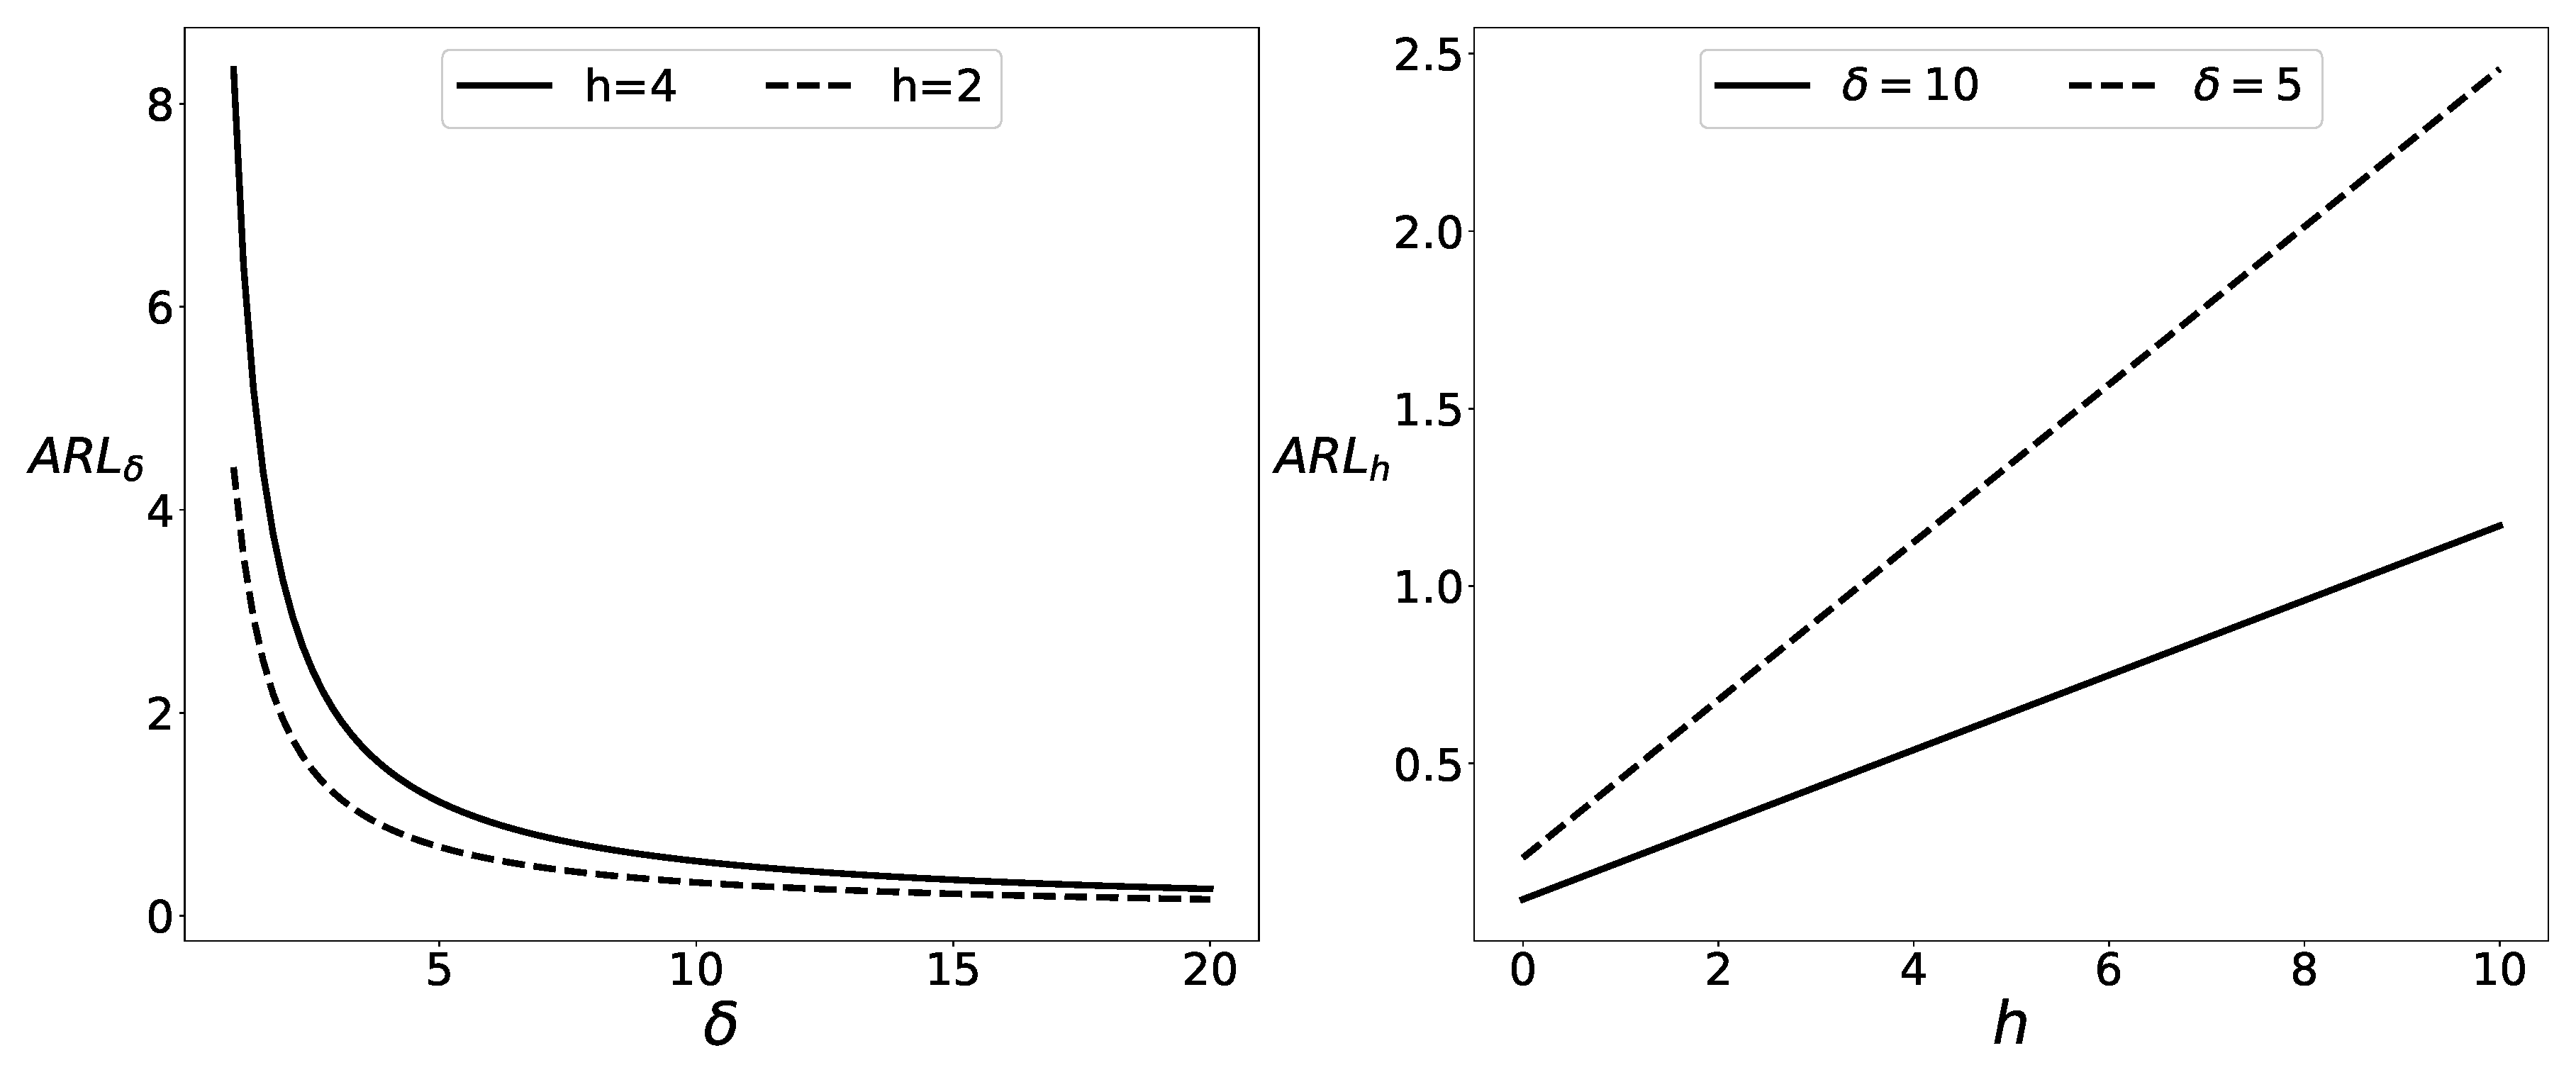
\includegraphics[width=0.9\textwidth]{pics/journal_paper/arl.eps}
	\caption{
    The left plot depicts ARL as a function of $\delta = \mu_2-\mu_1$ for two fixed threshold values $h$. The right plot depicts ARL as a function of the threshold value $h$ for two fixed $\delta$ values (Equation~\ref{eq:arl_approximation}).
    Both plots demonstrate that smaller ARL values (and therefore detection delays) correspond to smaller $h$ values. It is obvious for the right plot, on the left plot this fact is depicted by the dashed line for $h=2$ being lower than the solid line for $h=4$.
    %
    Smaller $\delta$ corresponds to the fluctuations in the time series causing false alarms, larger $\delta$ correspond to changes in the level shift which are subject for detection.
    When threshold $h$ is adjusted to smaller values ARL for all $\delta$ values gets smaller (left plot), therefore detection delay is decreased but probability of FA is increased.
    %Left plot depicts that ARL values for the whole range of $\delta$ values are decreased including smaller $\delta$ values corresponding to FA events,i.e.\ average runs between false alarms are also decreased along with the detection delay.
    %
    % Our hypothesis which we investigate experimentally is that by using smaller values of $h$ within prediction intervals and by disregarding detections outside of them we can decrease detection delay and the total number of false alarms despite decreased average runs between them.
}\label{fig:arl}
\end{figure}
% Plot on the right side of Figure~\ref{fig:arl} depicts ARL's values against
% threshold $h$ for two $\delta$ values.
% In a simplified form we can see that $\text{ARL} \sim \frac{\exp(-\delta)}{\delta^2}$.
% k=0.5, h=4 or 5 in \cite{el2018depth}


\subsection{Random walk property of CuSum output statistic}
In order to investigate how detection delay and false alarm rate depend on the detection threshold $h$ in static and dynamic settings, it is important to describe CuSum's statistical properties before and after a change point.
Assuming that the input signal before the change follows
$x_i \sim \mathbb{N}(\mu_0, \sigma)$
and after the change
$x_i \sim \mathbb{N}(\mu_0 + \delta, \sigma)$, the
CuSum's output statistic can be calculated as
$s_i = x_i - \mu_0$ if $i == 0$,
and as
$s_i = s_{i-1} + x_i - \mu_0$ if $i > 0$.
%
If $x_i \sim \mathbb{N}(\mu_0, \sigma)$ then
$x_i - \mu_0 \sim \mathbb{N}(\mu=0, \sigma)$
before the change, and, therefore, the CuSum's statistic
$s_i =s_{i-1} + x_i - \mu_0$ is a Gaussian random walk
$s_i = \sum_{i=0}^{k} (x_i \sim \mathbb{N}(\mu=0, \sigma))$.
Furthermore, after the change,
$x_i - \mu_0 \sim \mathbb{N}(\delta, \sigma)$
and, therefore, $s_i$ is a random walk with the drift.
%
So, before the change CuSum's output statistic behaves as a Gaussian random walk (RW) stochastic process and after the change as a random walk with the drift (see example on Figure~\ref{fig:possible_outcomes}).
Variance of the RW increases over time as a function of $\sigma \sqrt{t}$ with expected value staying around $0$.
Expected value of the RW with drift increases according to the linear trend $\sim t \mu$.
That is why ARL increases as it is depicted on the right plot of Figure~\ref{fig:arl} with increasing threshold value $h$ according to the Equation~\ref{eq:arl_approximation}.
It also becomes clear that false alarm events are caused not only by input signal properties but also by the stochastic nature of the CuSum's output statistic.
Even if there is no change point in the signal, there is still a non-zero probability of FA event.
This is depicted on the left plot in Figure~\ref{fig:arl} by large values of ARL corresponding to small values of $\delta$.
% https://en.wikipedia.org/wiki/Random_walk
% Figure~\ref{fig:arl},Equation~\ref{eq:arl_approximation}
% ? $Var(x_t) = t \sigma^2$
% ? ~\cite{billingsley2013convergence},~\cite{basseville1993detection}.
%
% False Alarm (FA) before actual change may be
% caused by the fact that RW value may cross any
% predefined threshold as it variance is increasing
% as $Var(x_t) = t \sigma^2$.  This is a well known
% property of the Brownian
% motion.
% A.R.L.~\cite{Page1954}.
% Cusum statistic can cross any threshold at any
% time moment with the increasing probability as
% time increases.  After the change it will cross
% the same threshold faster.

Let us comment Figure~\ref{fig:possible_outcomes} depicting Cusum's output statistic before and after a change point.
Figure depicts two detections, change point location in the middle, threshold value (horizontal line), and prediction intervals (ROI).
Depicted threshold value is not optimal on a global scale for the whole signal, but it is optimal locally in case if we use a prediction interval.
In this case the first detection, which is a false alarm, is skipped, while second detection is a correct detection with a smaller detection delay in comparison to the case where we would use larger $h$ on the global scale in order to skip false alarms.
This example demonstrates that despite the fact that by making threshold value smaller we decrease ARL values both for detection delay and for false alarms, according to the Figure~\ref{fig:arl} and Equation~\ref{eq:arl_approximation}, it is still possible to improve the performance both for detection delay and FA rate.
Smaller ARL imply higher probability of false alarms but number of false alarms can be lower in dynamic settings, because we consider subsets of the input signal which are within prediction intervals.
Plots in column B on Figure~\ref{fig:possible_outcomes} illustrates the opposite case when the performance is decreased when using the prediction interval (ROI).
Run length for detection after a change point happens to be longer than the ROI width. Other outcomes are possible which are discussed in detail in the Section~\ref{sec:performance} about performance metrics.

An important factor to note is that if we wouldn't have strict constraints on the detection delay to be that small as depicted on Figure~\ref{fig:possible_outcomes}, then the optimal strategy would be to just increase threshold value and it would result in zero FA rate and in a longer detection delay.
So, we consider optimality of change detection in the presence of prediction intervals when having constraints on the detection delay values.
\begin{figure}[!htb]
	\begin{minipage}[t]{1.0\textwidth}
    \centering
    % trim={<left> <lower> <right> <upper>}
    \includegraphics[width=0.44\textwidth, trim={1.5cm 1.0cm 0.3cm 1.0cm}]{pics/journal_paper/proof_of_concept2.eps}
    \includegraphics[width=0.44\textwidth, trim={1.5cm 1.0cm 0.3cm 1.0cm}]{pics/journal_paper/proof_of_concept2_fn_case.eps}
    \\
		\includestandalone[width=0.35\textwidth]{pics/journal_paper/tikz/perf_metrics_case1}
    \hspace{10mm}
		\includestandalone[width=0.35\textwidth]{pics/journal_paper/tikz/perf_metrics_case2}
		\caption{
    Left side plots depict how performance can be improved with prediction interval (ROI). 
    Detection 1 is false alarm and it is ignored since it is outside ROI. 
    Detection 2 is alarmed after the change point with a small delay. 
    Without ROI we would have to increase threshold in order to avoid FA, but in this case detection delay would increase.
    Right side plots depict the case when performance is decreased when using prediction. Prediction interval is correct but the width of the interval isn't enough to detect change within it what leads to FN event. 
    Plots at the bottom depict how performance metrics are calculated.
    In both cases FA event causes FN event.
    If detection happens after the change but outside ROI (right side) then it is counted as FA.
    %Left plot at the bottom - if detection happens before change then it is FA event causing also FN. If detection happens after change then this is a TP event with non-NaN detection delay.
    %Right side plot depicts situation when detection happens outside ROI causing FA and FN. 
    %Change is not detected and delay is assigned $\text{NaN}$ value.
    }~\label{fig:possible_outcomes}
	\end{minipage}
\end{figure}
%         % Start: Individual plots
%         \begin{figure}[htb!]
%         	\centering
%         	\includegraphics[width=0.9\textwidth]{img/proof_of_concept2.eps}
%         	\caption{
%             The case when performance is improved.
%             Detection 1 is a false alarm (FA).
%             ROI is a prediction interval.
%             Detection 2 is a detection alarmed after the change point with a small delay.
%             When using ROI we skipped FA event and detected change with a smaller delay.
%             Otherwise we would have to increase threshold in order to avoid FA, but in this case delay value would increase.
%         	}
%         	\label{fig:method_works}
%         \end{figure}
%         \begin{figure}[htb!]
%         	\centering
%         	\includegraphics[width=0.9\textwidth]{img/proof_of_concept2_fn_case.eps}
%         	\caption{
%             The case when performance is decreased when using prediction.
%             Prediction interval is correct but the width of the interval isn't enough to detect change within it, what leads to FN event.
%         	}
%         	\label{fig:method_doesnt_work}
%         \end{figure}
%         % End: Individual plots



\section{Pccf}~\label{sec:pccf}
If change points are expected to reoccur in the input signal, then this prior information can be used to approximate prediction time intervals, or regions of interest (ROI), where changes are most likely to appear in the future.
Once calculated, and if predictions are correct, then this information can further be used to reduce the false alarm rate of the change detection process, %at the least
and potentially to reduce detection delays too.
FA rate can be decreased just by disregarding detections outside prediction intervals, and the detection delay can be decreased by increasing sensitivity of the detector within prediction intervals.
But, as mentioned, if sensitivity is increased, then probability of FA events will also  increase.
Possibility of decreasing detection delays in the presence of prediction interval is a subject of Experiments section.
We describe next how to calculate prediction intervals for reoccurring change points.

To calculate ROIs for recurrent change points we use a prediction confidence change function (Pccf) proposed in our previous work~\cite{MaslovSDM2016}, where it was calculated using convolutions.
Below we calculate Pccf for several commonly used distributions of inter-arrival times values using moment generating functions, what is a more concise way than when using convolutions.
%~\footnote{we useterms recurrent and reoccurring interchangebly}
% The difference to the previous work is that we calculate Pccf in a concise
% way using moment generating functions and we calculate it for several
% commonly used distributions used for inter arrival time modelling.
%In our previous work we applied threshold value to the calculated probability estimates, but now we found it much more practical just to use equally spaced time moments surrounded by time intervals of a fixed size.
% Probability estimates given by Pccf should be used to assess confidence intervals for predictions and for assessment of how many changes in the future we want to make a prediction for.
Let's start with definitions.
\begin{definition}
	Change points $t_i^{\text{c}}$ are recurrent if their inter-arrival times $t_{i}^{c} - t_{i-1}^{c}$
  % \begin{equation}\label{eq:recurrence_relation}
  %     \Delta_i = t_{i}^{c} - t_{i-1}^{c}
  % \end{equation}
  are i.i.d.\ from the same probability distribution.
  E.g., $t_{i}^{c} - t_{i-1}^{c} \sim \mathbb{N}(\mu, \sigma)$ if $\sigma$ is small.
\end{definition}
%The recurrence relation for recurrent changes is
%\begin{equation} x_{n+1} = x_n + \delta_n \end{equation}
%
Pccf function value at time moment $t_i$ is a probability estimator of recurrent change point to occur at this time moment.
%Pccf function value at time moment $t_i$ is a probability estimation of the event of observing recurrent changepoint at this moment.
%Recurrent changepoints form a sequence determined by recurrence relation given by Equation~\ref{eq:recurrence_relation}.
% $t_{i}^{\text{CHP}} = t_{i-1}^{\text{CHP}} + \Delta_i$.
Pccf can be represented as a matrix~\ref{eq:pccf_matrix} in which elements at row $k$ and column $i$ are probability estimates for change point $t_k^{\text{c}}$ to appear at time moment $t_i$.
\begin{equation}~\label{eq:pccf_matrix}
	\text{PCCF}_{k,i} \equiv P(t_{k}^{\text{c}} = t_i) % \: \forall \:  k, i \in [1,\dots,N
\end{equation}
When calculating ROIs we are interested in total probability of any changepoint occurring at every time moment within prediction horizon.
Since events $t_k^{\text{c}} = t_i$ are disjoint we need to sum up rows of the matrix $\text{PCCF}_{k,i}$
\begin{equation}~\label{eq:pccf_vector}
  \text{PCCF}_{i \in 1:N} = \sum_{k=1}^{N} P(t_k^{\text{c}} = t_i) \equiv \sum_{k=1}^{N} \text{PCCF}_{k,i}
\end{equation}
Further by Pccf we call the vector given by Equation~\ref{eq:pccf_vector}.
 %, i.e.  $\sum_{k=1}^{N} P(t_k^{\text{CHP}} = t_i)$.
%	\begin{equation}
%		\text{Any } t_{k}^{\text{CHP}} = t_i
%		% \text{ or } t_{2}^{\text{CHP}} = t   \dots t_{k}^{\text{CHP}} = t
%		%C_1 = t \text{ or } C_2 = t \text{ or } \dots C_n = t
%		\label{eq:events_union}
%	\end{equation}
%Since events $t_k^{\text{CHP}} = t_i$ are disjoint Pccf can be calculated as
%\begin{equation}
%	\sum_{i=1}^{N} \sum_{k=1}^{N} P(t_k^{\text{CHP}} = t_i).
%\end{equation}
%\begin{equation}
%	P\Big(\bigcup\limits_{k=1}^{N} (t_k^{\text{CHP}} = t_i) \Big ) = \sum_{k=1}^{N} P(t_k^{\text{CHP}} = t_i)
%\end{equation} % Wasserman, page5

The sum~\ref{eq:pccf_vector} can be calculated using the notion of moment generating function (Mgf).
As an example, let's assume a Gaussian distribution for inter-arrival times, i.e. $t_{i}^{\text{c}} - t_{i-1}^{\text{c}} \sim \mathbb{N}(\mu, \sigma)$,
with $\sigma$ small enough so that every next change can not happen before the previous one.
For example, if $\mu=60$ seconds and standard deviation is $\sigma=5$ seconds then, using Chebyshev's inequality~\ref{eq:chebyshev_ineq}, probability of
$\mathbb{P}(|t_{i}^{\text{c}} - t_{i-1}^{\text{c}}| \geq 60) \leq 0.007$.
\begin{equation}\label{eq:chebyshev_ineq}
	\mathbb{P}(|X-\mu| \geq k \sigma) \leq \frac{1}{k^2} % %\mathbb{P}(|X-\mu| \geq t) \leq \frac{\sigma^2}{t^2}
\end{equation}
%\subsec{Predicting sequential events}
% Resources
% \href{https://www.youtube.com/playlist?list=PL2SOU6wwxB0uwwH80KTQ6ht66KWxbzTIo}{Statistics 110: Probability}
%- [lec24] [Lecture 24: Gamma distribution and Poisson process](https://www.youtube.com/watch?v=Qjeswpm0cWY&index=24&list=PL2SOU6wwxB0uwwH80KTQ6ht66KWxbzTIo)
%- [lec22] [Lecture 22: Transformations and Convolutions](https://www.youtube.com/watch?v=yXwPUAIvFyg&list=PL2SOU6wwxB0uwwH80KTQ6ht66KWxbzTIo&index=22)
%- [lec17] [Lecture 17: Moment Generating Functions](https://www.youtube.com/watch?v=N8O6zd6vTZ8&index=17&list=PL2SOU6wwxB0uwwH80KTQ6ht66KWxbzTIo)
%- [lec18] [Lecture 18: Mgfs Continued](https://www.youtube.com/watch?v=tVDdx6xUOcs&list=PL2SOU6wwxB0uwwH80KTQ6ht66KWxbzTIo&index=18)
%- [math.tntech.edu: Sum of independent random variables](http://math.tntech.edu/ISR/Introduction_to_Probability/Distributions_of_Functions/thispage/newnode11.html)
%- [Table of Common Distributions](http://www.stat.tamu.edu/~twehrly/611/distab.pdf) taken from Statistical Inference by Casella and Berger
%The sum~\ref{eq:pccf_sum} can be calculated by calculating Mgf of the sum of i.i.d.\ variables and after that by pattern\ - similarity to the Mgf of individual variable find the PDF of the sum.
%\begin{definition}
By definition, Mgf, or Laplace transform, of random variable $X$ is~\ref{eq:mgf}
%~\footnote{Mgf is $\mathbb{E}(e^{tX})$ while characteristic function is $\mathbb{E}(e^{i t X})$.}
\begin{equation}\label{eq:mgf}
    M_{X}(t) = \mathbb{E}(e^{t X}), \: t \in \mathbb{R}
\end{equation}
%\begin{equation}~\label{eq:mgf}
%	%\psi_{X}(t) = \mathbb{E}(e^{t X}) = \int e^{tX} d F(x)
%	M_{X}(t) = \mathbb{E}(e^{t X})
%\end{equation}
% Moments of a distribution is computed as $\psi^{(k)} (0)=\mathbb{E}(X^k)$.
% Mgfs is a convenient tool to obtain distribution of sums of random variables.
Using the property that expected value of the product of two independent random variables is the product of their expected values $\mathbb{E}(X \dot Y)=\mathbb{E}(X)\mathbb{E}(Y)$, Mgf of the sum of independent random variables is a product of individual Mgfs (Equation~\ref{eq:mgf_of_sum}).
\begin{equation}\label{eq:mgf_of_sum}
	M_{X+Y}(t) = \mathbb{E}(e^{t (X+Y)}) = \mathbb{E}(e^{t X}) \mathbb{E} (e^{t Y}) \equiv M_{X}(t) M_{Y}(t)
\end{equation}
For the Gaussian distribution Mgf is $\exp{(\mu t + \frac{\sigma^2 t^2}{2})}$ and therefore
\begin{equation}\label{eq:mgf_gauss}
  M_{X+Y}^{\text{Gaussian}}(t)  = \exp \Big ((\mu_X + \mu_Y) t + \frac{(\sigma_X^2 + \sigma_Y^2) t^2}{2} \Big )
  % M_{X+Y}^{\text{Gaussian}}(t)  = \exp \Big [ (\mu_X + \mu_Y) t + \frac{(\sigma_X^2 + \sigma_Y^2) t^2}{2} \Big ]
\end{equation}
But~\ref{eq:mgf_gauss} is Mgf of the Gaussian distribution with parameters $\mu=\mu_1+\mu_2$ and $\sigma=\sqrt{\sigma_X^2 + \sigma_Y^2})$.
Therefore if probability distribution of the first change point is $t_1^{\text{c}} \sim \mathbb{N}(\mu, \sigma)$ then $t_2^{\text{c}} \sim \mathbb{N}(2\mu, \sigma \sqrt{2})$, etc.
And Pccf is a sum~\ref{eq:pccf_gaussian}
\begin{equation}\label{eq:pccf_gaussian}
    \text{PCCF}^{\text{Gaussian}} \equiv \sum_{k=1}^N \mathbb{N}(k \mu, \sqrt{k} \sigma)
\end{equation}
% Mgfs for commonly used for inter-arrival times modelling distributions are~\cite{wasserman2013all}
% as follows.
% for Exponential distribution with rate $\lambda$ it is $\frac{\lambda}{\lambda - t}$;
% and for the Gamma distribution $\Gamma(\alpha, \lambda)$ is $\Big ( \frac{1}{1- \lambda t} \Big )^{\alpha}$.
	% $\Big (\frac{\lambda}{\lambda - t} \Big)^{\alpha}$ %([ref](http://math.tntech.edu/ISR/Introduction_to_Probability/Distributions_of_Functions/thispage/newnode11.html))
	%
	% % POSISSON is not needed, as we model inter-arrival times, not number of occurences
	%\item Poisson is $e^{\lambda (e^t-1)}$
	%
	% $\mathbb{E}(e^{tX}) = \sum_{k=0}^{\infty} e^{tk} e^{-\lambda} \lambda^k/k! = e^{\lambda (e^t-1)}$
% https://en.wikipedia.org/wiki/Gamma_distribution#Summation
% https://stats.stackexchange.com/questions/51605/the-sum-of-two-independent-gamma-random-variables
% proof: https://en.wikipedia.org/wiki/Characteristic_function_%28probability_theory%29#Example
%Proof for the Gamma can be found \href{https://en.wikipedia.org/wiki/Characteristic\_function\_\%28probability\_theory\%29#Example}{here}. Characteristic functions are $\phi_X(t)=(1-\lambda i t)^{-a}$ and $\phi_Y(t)=(1-\lambda i t)^{-b}$. Therefore $\phi_{X+Y}(t) = (1-\lambda i t)^{-(a+b)}$.
%
% Poisson & $\mathbb{E}(e^{tX}) = \sum_{k=0}^{\infty} e^{tk} e^{-\lambda} \lambda^k/k! = e^{\lambda (e^t-1)}$ & Inter-arr. times are from Exp. And Pdf is for Gamma \\
%Weibull? & & p pp\\
% Gamma~\cite{wasserman2013all}
%
%  Corresponding Mgfs for the sums are as follows.
%  for Gamma distribution $M_{X+Y} (t) =  \Big (\frac{\lambda}{\lambda - t} \Big)^{a + b}$
%  and for Exponential distribution is $\frac{\lambda}{\lambda-t}$.
%
%  Gaussian,
%  If $X \sim N(\mu_X, \sigma_X)$ and $Y \sim N(\mu_Y,\sigma_Y)$ then $X+Y \sim N(\mu_X + \mu_Y, \sqrt{\sigma_X + \sigma_Y})$
%  $$M_{X+Y}(t) = \exp \Big ( t \mu_X  + \frac{\sigma_X^2 t^2}{2} \Big) \cdot \exp \Big ( t \mu_Y  + \frac{\sigma_Y^2 t^2}{2} \Big) = \exp \Big [ (\mu_X + \mu_Y) t + \frac{(\sigma_X^2 + \sigma_Y^2) t^2}{2} \Big ] $$ which is a characteristic function of the normal distribution with parameters $\mu =  \mu_X + \mu_Y$ and $ \sigma^2 = \sigma_X^2 + \sigma_Y^2$.
%
%
% $\Gamma(k, \lambda)$.
% Copied to for)thesis.tex
%
%\begin{itemize}
%	% POSISSON is not needed, as we model inter-arrival times, not number of occurences
%	%    %\item \textbf{For the Poisson.}
%	%$$M^P_{X+Y} (t) =  e^{\lambda (e^t-1)}  e^{\mu (e^t-1)} =  e^{(\lambda+\mu) (e^t-1)}$$
%	%It means $X+Y \sim \text{Poiss}(\lambda + \mu)$ (note: the sum of two Poissons is also a Poisson, which is not general for any distribution)
%	\item \textbf{Gaussian}
%	If $X \sim N(\mu_X, \sigma_X)$ and $Y \sim N(\mu_Y,\sigma_Y)$ then $X+Y \sim N(\mu_X + \mu_Y, \sqrt{\sigma_X + \sigma_Y})$
%	$$M_{X+Y}(t) = \exp \Big ( t \mu_X  + \frac{\sigma_X^2 t^2}{2} \Big) \cdot \exp \Big ( t \mu_Y  + \frac{\sigma_Y^2 t^2}{2} \Big) = \exp \Big [ (\mu_X + \mu_Y) t + \frac{(\sigma_X^2 + \sigma_Y^2) t^2}{2} \Big ] $$
%
%	which is a characteristic function of the normal distribution with parameters $(\mu =  \mu_X + \mu_Y, \sigma^2 = \sigma_X^2 + \sigma_Y^2)$.
%
%	\item \textbf{Gamma}
%	If $X \sim \Gamma(a, \lambda), Y \sim \Gamma(b, \lambda)$ then $X+Y \sim \Gamma(a+b, \lambda)$.
%
%	$$M_{X+Y} (t) = M_X (t) \cdot M_Y (t) = \Big (\frac{\lambda}{\lambda - t} \Big)^{a}  \Big (\frac{\lambda}{\lambda - t} \Big)^{b} =  \Big (\frac{\lambda}{\lambda - t} \Big)^{a + b}$$
%
%	\item \textbf{Exponential}
%	Mgf for the exponential distribution with $\lambda=1$ is $\frac{1}{1-t}$ where $t<1$.
%	% Lec.14 (Statistics 101): https://www.youtube.com/watch?v=Qjeswpm0cWY&index=24&list=PL2SOU6wwxB0uwwH80KTQ6ht66KWxbzTIo
%	% START: 23:27
%	% Using the property of moment generating functions (by definition)
%	% \[\psi_{X+Y}(t) = \mathbb{E}(e^{t (X+Y)}) = \mathbb{E}(e^{t X}) \mathbb{E} (e^{t Y})\]
%	Mgf for the $n$-th event $T_n = \sum_{j=1}^{n} X_j, \text{ where } X_j \sim e^{-\lambda t}$ is $\Big ( \frac{1}{1-t} \Big )^n$.
%	But Mgf for $Y \sim \Gamma(n,1)$ is also $\Big(\frac{1}{1-t} \Big)^n$.
%	Therefore if inter-arrival times are i.i.d. from the exponential distribution with parameter $\lambda$ the PDF for the k-th event is $\Gamma(k, \lambda)$.
%	%\begin{equation}
%	%    \mathbb{E}(e^{tY}) = \frac{1}{\Gamma(n)} \int_{0}^{\infty} e^{ty} y^{n} e^{-y} \frac{d y}{y} = \frac{1}{\Gamma(n)} \int_{0}^{\infty} y^n e^{-(1-t)y} \frac{d y}{y}
%	%\end{equation}
%	%Let, $x=(1-t)y$, then $d x = (1-t) d y$, then we get
%	%\begin{equation}
%	%    \mathbb{E}(e^{tY}) = \frac{(1-t)^{-n}}{\Gamma(n)} \int_{0}^{\infty} x^n e^{-x} \frac{d x}{x} = \Big(\frac{1}{1-t} \Big)^n
%	%    \label{eq:mgf_gamma_1}
%	%\end{equation}
%	%This is (Equation~\ref{eq:mgf_gamma_1}) the same Mgf as Mgf for the sum of i.i.d. from Exponential distribution with $\lambda=1$ (Equation~\ref{eq:mgf_exp_n}).
%
%	%If $X \sim Exp(\lambda_1)$ and $Y \sim Exp(\lambda_2)$ then $X+Y \sim $
%	%$$M^E_{X+Y}(t) = \frac{\lambda_1}{\lambda_1 - t} \frac{\lambda_2}{\lambda_2 - t}$$
%\end{itemize}

Using the same logic it is straightforward to calculate Pccfs for Exponential and Gamma distributions (Table~\ref{table:pccfs}).
\begin{table}[!htb] \caption{Pdf's for distributions of inter-arrival times.}\label{table:pccfs}
	\begin{center}
		\begin{tabular}{|l|l|c|c|}
			\hline
			Distribution & Mgf & PDF of the $k$-th event & PCCF  \\[5pt]
			\hline
			Gaussian & $\exp{ (\mu t + \frac{\sigma^2 t^2}{2}) }$ & $\mathcal{N}(k \mu, \sqrt{k} \sigma)$ & $\sum_{k=1}^N \mathcal{N}(k \mu, \sqrt{k} \sigma)$ \\
			Gamma $\Gamma(\alpha, \lambda)$ & $\Big ( \frac{1}{1- \lambda t} \Big )^{\alpha}$ & $\Gamma(k \alpha, \lambda)$ & $\sum_{k=1}^N \Gamma(k \alpha, \lambda)$\\
			Exponential & $\frac{\lambda}{\lambda - t}$ & $\Gamma(k, \lambda)$ & $\sum_{k=1}^N \Gamma(k, \lambda)$\\
			\hline
		\end{tabular}
	\end{center}
\end{table}
%In the paper~\cite{MaslovSDM2016} we considered a Gaussian distribution instead of, for example, Gamma distribution assuming that standard deviation ``$\sigma$ is small enough'' so that we can neglect probabilities of the events in the negative values tail of the distribution.
%Markov's inequality.63~\cite{wasserman2013all}.p.249~\cite{feller2008introduction}: if $X$ is a non-negative random variable, then $\forall t >0$
%\begin{equation}
%	\mathbb{P}(X>t) \leq \frac{\mathbb{E}(X)}{t}
%	\label{eq:markov_ineq}
%\end{equation}
%Chebyshev's inequality: let $\mu=\mathbb{E}(X)$ and $\sigma^2=\mathbb{V}(X)$ then,
Figure~\ref{fig:pccf_example} depicts Gaussian Pccf.
Prediction intervals (ROI) can be calculated by applying a threshold value for Pccf and then ROIs will be determined by time moments when Pccf exceeds this threshold.
In this way we would take into account uncertainty in the predictions for $k$-th change points which will increase as $\sqrt{k} \sigma$ (Equation~\ref{eq:pccf_gaussian}).
Another way is to use the property that Pccf extremums are equally spaced (Equation~\ref{eq:rois})~\cite{MaslovSDM2016} by time intervals $\mu$.
After estimating $\mu$ between changes and choosing the number of change points $k$ to predict and ROIs width prediction interval are determined by Equation~\ref{eq:rois}.
\begin{equation}\label{eq:rois}
  \text{ROI}s = (\mu \pm \text{ROI}_{\text{Width}}, 2 \mu \pm \text{ROI}_{\text{Width}}, \dots , k \mu \pm \text{ROI}_{\text{Width}}).
\end{equation}
\begin{figure}[htb!]
	\centering
	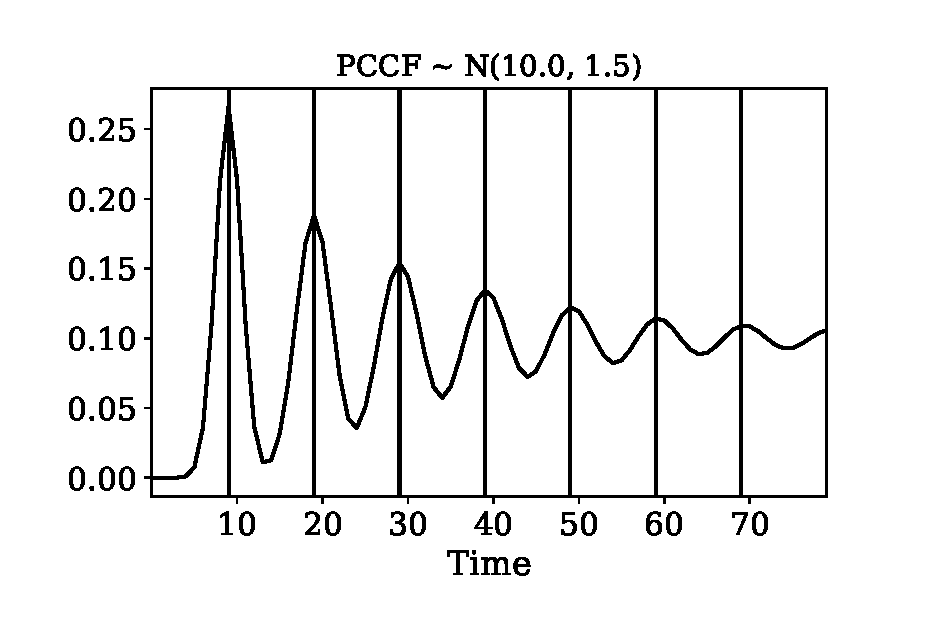
\includegraphics[scale=0.5]{pics/journal_paper/pccf_example.eps}
	\caption{
    Gaussian PCCF.
		The oscillating curve depicts probability estimation for the changepoint to occur at corresponding time moment.
		Peaks are located at time moments $(\mu, 2 \mu, 3\mu, \dots)$.
		% Given this observation in experiments we use naive version of Pccf which is a vector of prediction intervals (ROIs) $k \mu \pm \delta, k = 1,2,...$
	}
	\label{fig:pccf_example}
\end{figure}
% Since Pccf decreases its values while oscillating and converging to the constant value over time we effectively choose first $k$ peaks of Pccf by applying threshold.
%By observing how fast Pccf converges to the constant level we can select $k$ based on visual inspection of Pccf behavior.
%Then we would need to select how many change points we need to predict
%After that ROI intervals can be allocated around Pccf's local extremums


\section{Performance metrics}~\label{sec:performance}
As mentioned in Section~\ref{sec:cusum_detector}, the commonly used change detection performance metric with Cusum is the ARL value, which refers to the FA rate before change point and to the detection delay after the change.
% When the process is in-control, $ARL_{\delta}$ refers to FA rate, when the
% change has happened it refers to the response time/detection delay.
% On the Figure\ref{fig:arl} the first case corresponds to small $\delta$ values, e.g.\ noise in the signal, and the second case to larger values when $\delta \sim \mu_2 - \mu_1$.
% As the our goal is to reduce detection delay while keeping FA rate the same or lower by using prediction intervals, the fact that ARL refers to two types of errors at the same time makes it not sufficient to describe and compare performance of dynamic and static detectors accurately.
In case of multiple change points, the ARL metric is not sufficient as it doesn't reflect how many changes were detected and missed.
As in~\cite{bodenham2017continuous} and in~\cite{plasse2021streaming}, in addition to the detection delay, we use binary classification metrics to assess performance of the change detection process.
We define those metrics in terms of mappings between change and detection events as follows.
\begin{definition}
	We define TP, FA, FN and TN events in terms of mappings between change points and detections.
	To every TP corresponds one change point.
	FA is the detection to which there is no any corresponding change point.
	FN is change point to which there is no corresponding detection.
	More formally
	\begin{itemize}
    \item \textit{TP is a first detection (DE) after change point.} E.g., if $\text{changes}=[100], \text{DEs}=[50, 110, 121]$ then TP is $\text{d} =110$.

    \item \textit{Detection delay is a time interval between TP and corresponding change point} $t_{\text{d}} - t_{\text{c}} \geq 0$. If detection doesn't happen $\text{NaN}$ value is assigned to the delay.

    \item \textit{FA is a detection before change point or detection after another detection which was TP but before next change point.} E.g., if $\text{changes}=[100], \text{DEs}=[50, 110, 121]$ then FA are $\text{DEs} = [50, 121]$.

    \item \textit{FN is an event when there is no detection corresponding to the change point.} E.g., if $\text{changes}=[100, 150], \text{DEs}=[50, 110, 121]$ then FN is $[150]$. FN can be caused by events 1) Cusum output statistic didn't exceed threshold $h$ 2) in the dynamic case - if DE was alarmed after change point but not within prediction interval. E.g., if $\text{changes}=[100], \text{DEs}=[50, 121]$, prediction interval is $\text{ROI}=[(90, 110)]$ then FN is change point $[100]$.

    \item \textit{TN is every event when detection is not alarmed correctly}, i.e. - if alarmed it would cause FA.
		%??In a sequential change detection settings number of TN is constant value equal to the length of the signal $N$ minus sum of true positives and false positives: $TN=N - (TP+FA)$
		% But this is hard to calculate number of such events in a meaningful way in case of online change detection process and in terms of mappings between CDEs and changepoints.

\end{itemize}
\end{definition}
Figure~\ref{fig:possible_outcomes} illustrates given definitions for static and dynamic settings. As in~\cite{plasse2021streaming} we use $F_1=\frac{TP}{TP+\frac{1}{2}(FA+FN)}$ score metric combining precision and recall to measure detection performance along with the detection delay value.
There is a similarity to binary classification but analogy is not full because any change in real signal takes time.
And therefore all time moments and observations within change time interval should be labelled as change.
During change detection using CuSum no labels to observations or time moments are assigned.
CuSum alarms detection when its output statistic exceeds threshold.
%%%%%%%%
%The on-line change detection problem is to detect the change (or changes) as soon as possible with a fixed false alarm (FA) rate, i.e.\ to minimize the detection delay given a desirable FA rate ~\cite{basseville1993detection}.
% Section 1.1.2.1
%As mentioned in Section (Cusum) - ARL
%Commonly use performance metrics are 1) mean detection delay, probabilities 2) of false alarm (FA), 3) of false positive detection (FA) and 4) of nondetection, i.e.\ false negative (FN).
% Sec 1.1.2.4
% 1. mean time between FA
% 2. probability of false detection
% 3. mean delay for detection
% 4. probability of nondetection
% 5. accuracy of the change time and magnitude estimates
%For prediction step use $F_{1}$ score metric $F_1=\frac{TP}{TP + \frac{1}{2} (FP+FN)}$.
%
% %% START: Join with cusum statistic plots
% \begin{figure}[!htb]
% 	\centering
% 	\begin{minipage}[t]{0.9\textwidth}
% 		\centering
% 		\includestandalone[width=0.45\textwidth]{./tikz/perf_metrics_case1}
% 		\includestandalone[width=0.45\textwidth]{./tikz/perf_metrics_case2}
% 		\caption{
%     Plot A) - the case without prediction interval.
%     If detection happens before changepoint then it is FP event causing also FN.
%     If detection happens after change then this is a TP event with not NaN detection delay.
%     Plot B) - the case with the prediction interval (ROI).
%     Additional outcome is when detection happens outside ROI causing FP and FN.
%     If change is not detected than delay is assigned NaN value in experiments.
% 		}
% 		\label{fig:perf_metrics_case1}
% 	\end{minipage}
% \end{figure}
% %% END: Join with cusum statistic plots


\section{Experiments}\label{sec:experiments}
We perform two experiments to show how CuSum detection performance can be improved with prediction intervals. 

\subsection{Implementation}\label{sec:implementation}
Before the experimental results, we describe how the combination of Pccf in Section~\ref{sec:pccf} and the CuSum detector in Equations~\ref{eq:cusum_scheme} is translated to a change point detection framework.
The implementation is depicted in Algorithm~\ref{alg:method_code}.
%There, the function $CusumSingle$ implements a single change point detection and $CusumMulti$ implements a sequential change detection, correspondingly.
%$CusumMulti$ is an extended version of $CusumSingle$.
%In case of a single change point, their output is identical.
%$CusumSingle$ is presented for clarity since $CusumMulti$ contains additional logic to track the visited ROI intervals and to re-initialize the detector parameters after each detection.
The core logical part is a code snippet:
\begin{algorithm}[!h]
	\begin{algorithmic}
    \If{(not PCCF) or (PCCF and WithinRoi()) }
        \If{$|stat[t]| > h$}
            \State detections.append(t)
            \State ResetDetector()
        \EndIf
    \EndIf
	\end{algorithmic}
\end{algorithm}

\noindent
which states that the CuSum stopping rule is checked continuously if no prediction intervals (ROIs) are provided or checked only within ROI intervals if they are available. If so, the detection is collected to the array  and detector's settings are re-initialized. In case of a sequential change detection a new in-control mean value of the input signal is estimated using function $UpdateMu$ after each detection. An important property of the implementation is that  when detection happens before change point or does not happen at all then detection delay has NaN value (lines 17-18, Algorithm~\ref{alg:method_code}). And delay mean value is calculated after removing NaN values.
%Other options might be to return negative, or $\infty$ values, but in that case we wouldn't be able to calculate average delay.


\subsection{Artificial signal simulation}
In the first experiment we perform a simulation to measure average values of the detection delay and $F_1$ score of the CuSum detector in the presence of prediction interval and without it. We will measure performance while variating detection threshold $h$ and level shift in the mean value $\delta=\mu_2-\mu_1$, controlling signal-to-noise ratio. These two parameters are controlling ARL value (Figure~\ref{fig:arl}, Equation~\ref{eq:arl_approximation}).
We expect to see performance gain in dynamic case for small $h$ values when corresponding ARL is smaller or equal to the $\text{ROI}_{\text{Width}}$. For larger $h$ values detection will happen outside ROI (Figure~\ref{fig:possible_outcomes}) and static detector should perform better. 

Input signal was generated $1000$ times by drawing samples from Gaussian distribution with parameters $\mu_1=0, \sigma=1$ before change at time moment $t^c = 100$ and $\mu_2 \in [1.1, 2.1, 3.1], \sigma=1$ after change.
Prediction interval of width $\text{ROI}_{\text{Width}}=50$ is located in the middle of the signal symmetrically to the changepoint.
Performance metrics are measured while changing detection threshold value $h$ and signal level shift $\delta$.
Level shift $\delta$ is being increased in order to decrease corresponding ARL (Figure~\ref{fig:arl}, Equation~\ref{eq:arl_approximation}) and its ratio to the $\text{ROI}_{\text{Width}}$.
When ARL becomes larger we expect to see less performance gain when using dynamic settings since static detector will be able to detect change with similar delay.

Figure~\ref{fig:artificial_signal_perf_results} depicts the results.
Plots on the left side show averaged detection delays.
Plots on the right side show averaged $F_1$ score values.
Three rows of plots from top to down depict cases for different $\delta$ values.
Both in case of dynamic and static detector settings, when $h$ is small the detection delay is also small but there are a lot of false alarms. 
When threshold increases $F_1$ score increases because of fewer FA and the detection delay gets bigger. 

Detection delay with prediction interval is lower or the same as in case without prediction interval for all $h$.
Dashed curve depicting dynamic detector delays is shorter that solid curve corresponding to the static detector because because dynamic detection delay can't exceed half of the $\text{ROI}_{\text{Width}}$ (since ROI is symmetrical to change point location). 
In case of FA event detection delay is assigned to $\text{NaN}$ value. 
While calculating average value $\text{NaN}$ values are ignored. 
Therefore detection delay plot depicts only successful detections cases. 
The cases when delay is $\text{NaN}$ are captured by FA and FN factors in $F_1$ score value.

Dynamic CuSum $F_1$ score outperforms static CuSum (Figure ~\ref{fig:artificial_signal_perf_results}) for smaller $h$ values when false alarms outside ROI are skipped and change is detected within ROI. 
This situation is depicted on the left side of Figure~\ref{fig:possible_outcomes}.
When $h$ increases CuSum ARL exceeds $\text{ROI}_{\text{Width}}$ and detection doesn't happen within ROI.
This is depicted on the right side of Figure~\ref{fig:possible_outcomes}. 
%A this moment $F_1$ of static CuSum starts exceeding dynamic $F_1$ on the Figure~\ref{fig:artificial_signal_perf_results}.
%Average $F_1$ for dynamic case is higher than in static case up until the moment.This moment corresponds to the situation depicted on Figure~\ref{fig:possible_outcomes} (right side) When ARL of dynamic detector exceeds $\text{ROI}_{\text{Width}}$. 
% After some critical $h$ value detection in dynamic case is either happens within prediction interval or doesn't happen at all what results in FN and FA detections (Figure~\ref{fig:possible_outcomes}).
% Dynamic CuSum outperforms static settings CuSum in terms of detection delay and $F_1$ score values for smaller $h$.
\begin{figure}[!htb]
	\centering
	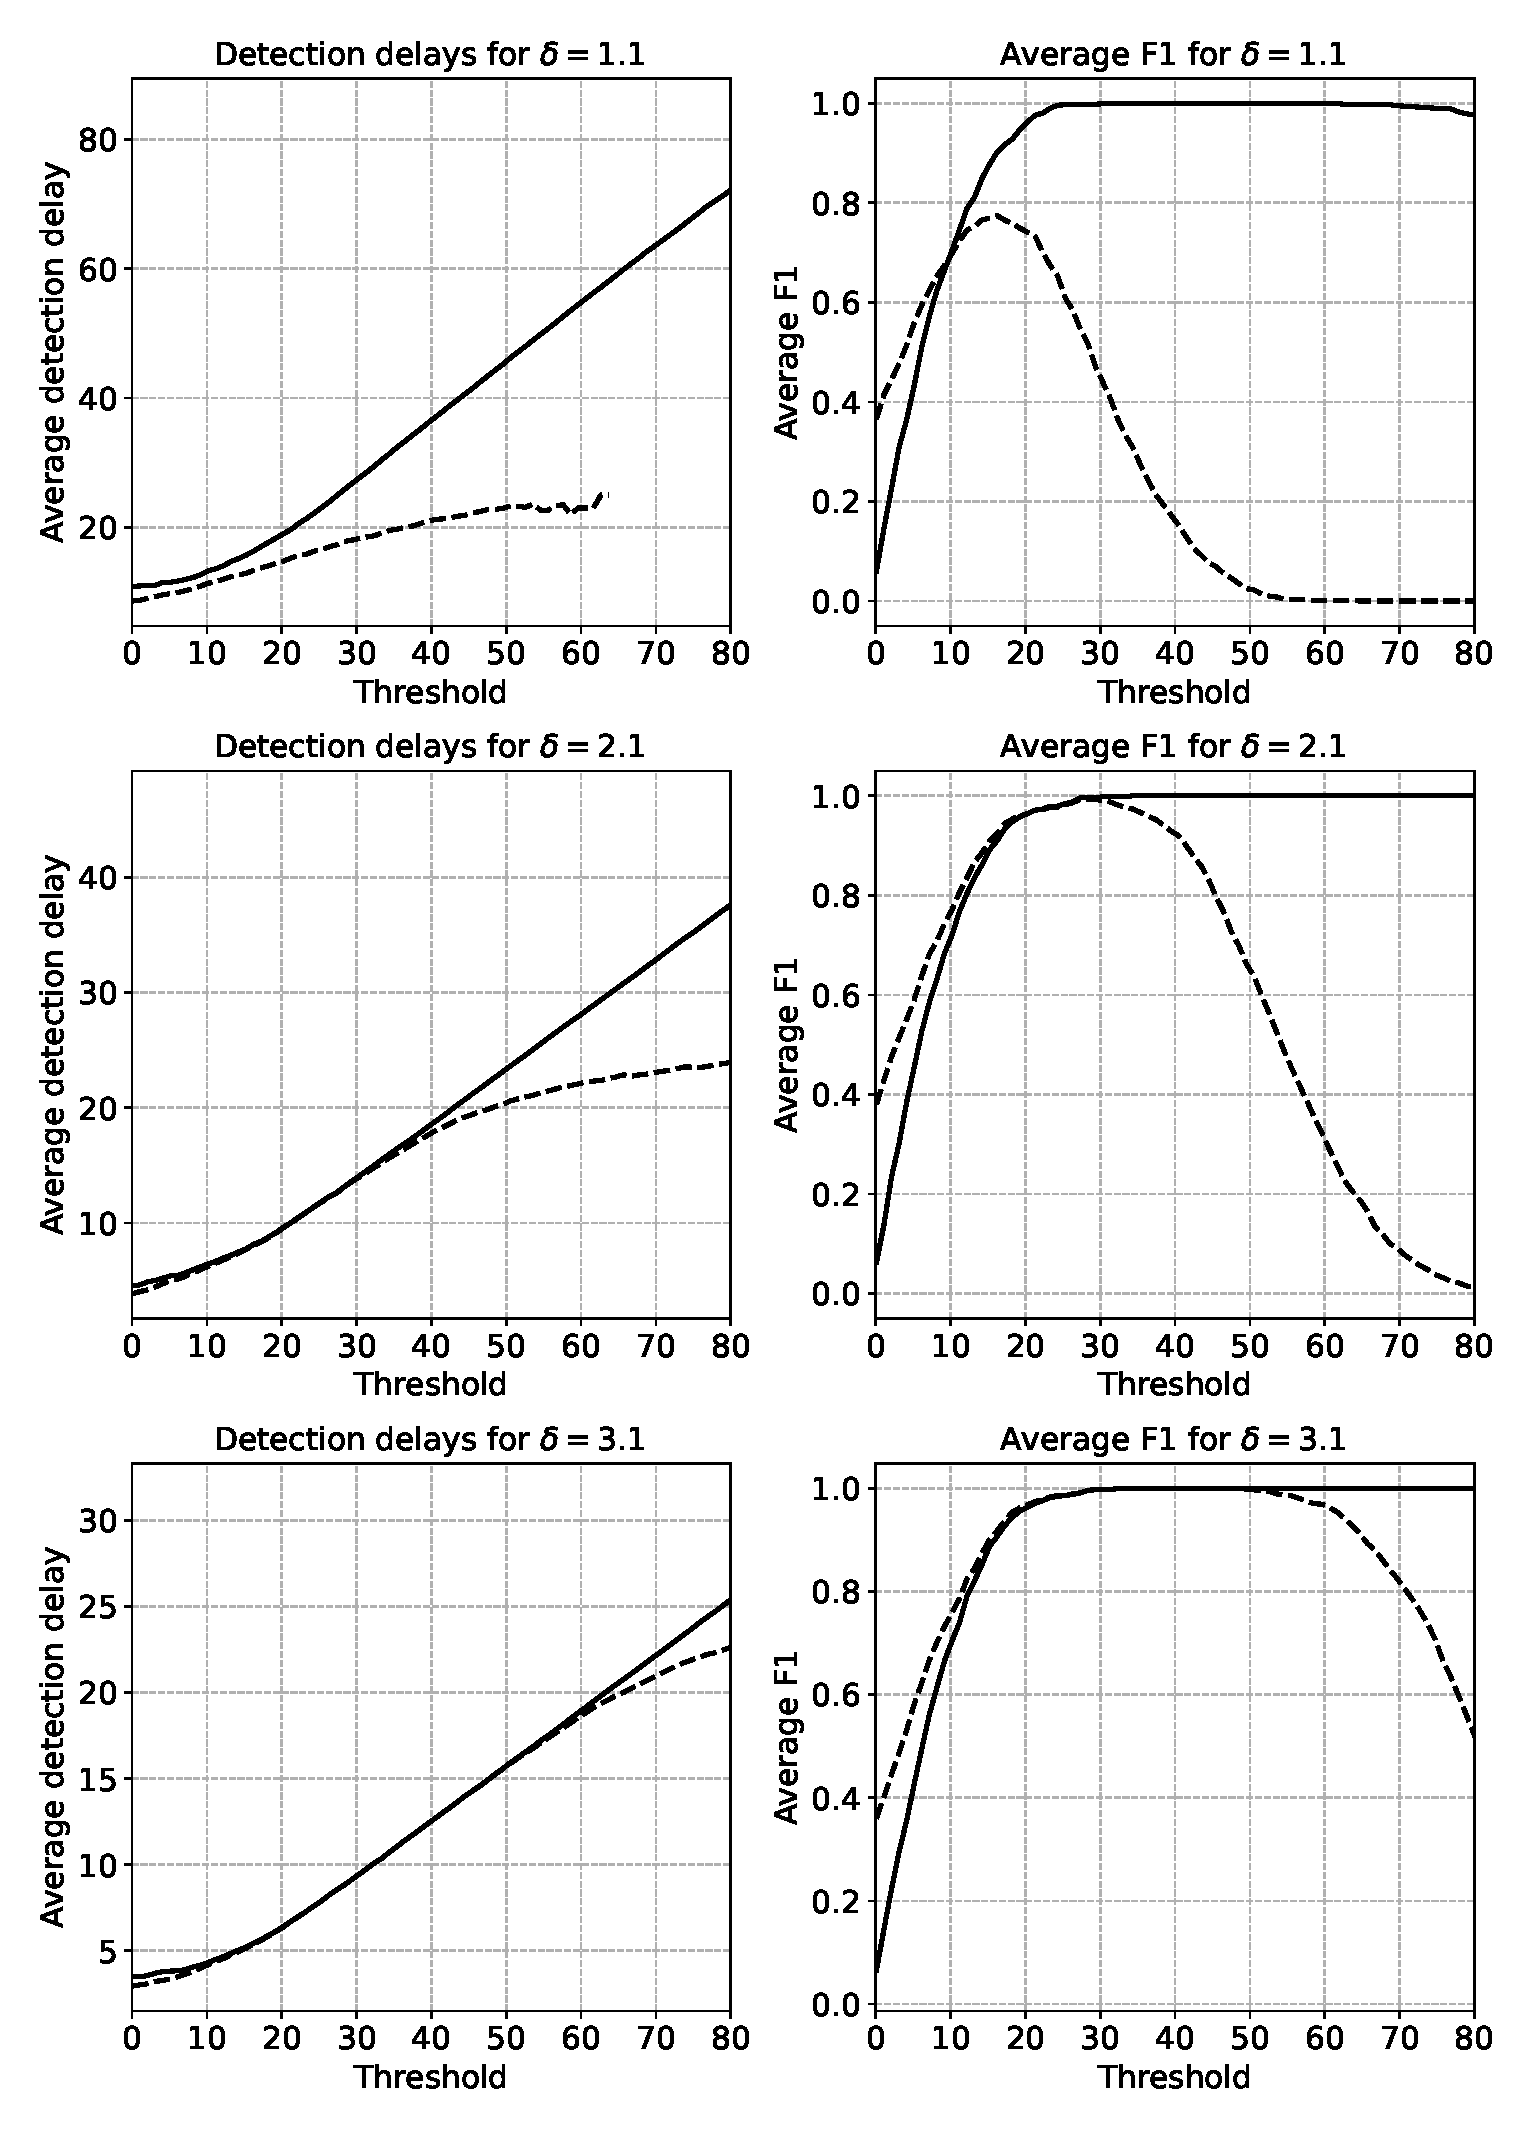
\includegraphics[width=0.90\textwidth]{pics/journal_paper/performance_detection_sim}
	\caption{Average detection delays (left side) and average $F_1$ score (right side) when variating threshold value $h$ (x-axis).
	Top, middle and bottom rows of plots are for different $\delta = \mu_2 - \mu_1$ values.
	Solid and dashed lines depict static and dynamic cases.
    Average delay is calculated after ignoring NaN values caused by FA.
    NaN delay values and corresponding FA events are counted by $F_1$.
    For small $h$ values corresponding to smaller ARL values comparable to the prediction interval width, dynamic CuSum performance is better.
    When $h$ gets larger static detector $F_1$ score starts exceeding dynamic detector curve.
    Detection delay plots depict only cases when FA event didn't happen, therefore it should be analyzed along with $F_1$ metric.
    Dynamic CuSum has better performance with the given ROI for $h$ values when $F_1$ dashed curve (dynamic case) is above solid curve (static case).
	}
	\label{fig:artificial_signal_perf_results}
\end{figure}


\subsection{Temperature data}
In the second experiment, we predict and detect multiple change points in the time series of temperature measurements collected from the sensor installed in the home office environment.
We measure the same performance metrics, except ARL, as in the first experiment when trying to predict all changes using Pccf and when predicting only several most earliest change points.
In the second experiment, we confirm results obtained in the first experiment using the real signal and, in addition, we investigate sensitivity of the results with regard to the prediction accuracy when calculating prediction intervals using Pccf.
An important difference also is that in this experiment we do not average detection delay values and therefore we also compare detection delays in static and dynamic cases directly without possibility to disregard $NaN$ values due to averaging.
Measurements took place in the city of Jyv\"{a}skyl\"{a} (Finland) from 06 Mar 2021 (19:11m) until 21 Mar 2021 what is a cold period in Finland.
Subject for the change detection is the beginning of every working day when heater was turned on in the morning and what caused abrupt changes in the ambient temperature.
Figure~\ref{fig:dht22} illustrates the measuring device.
\begin{figure}[htb!]
	\centering
	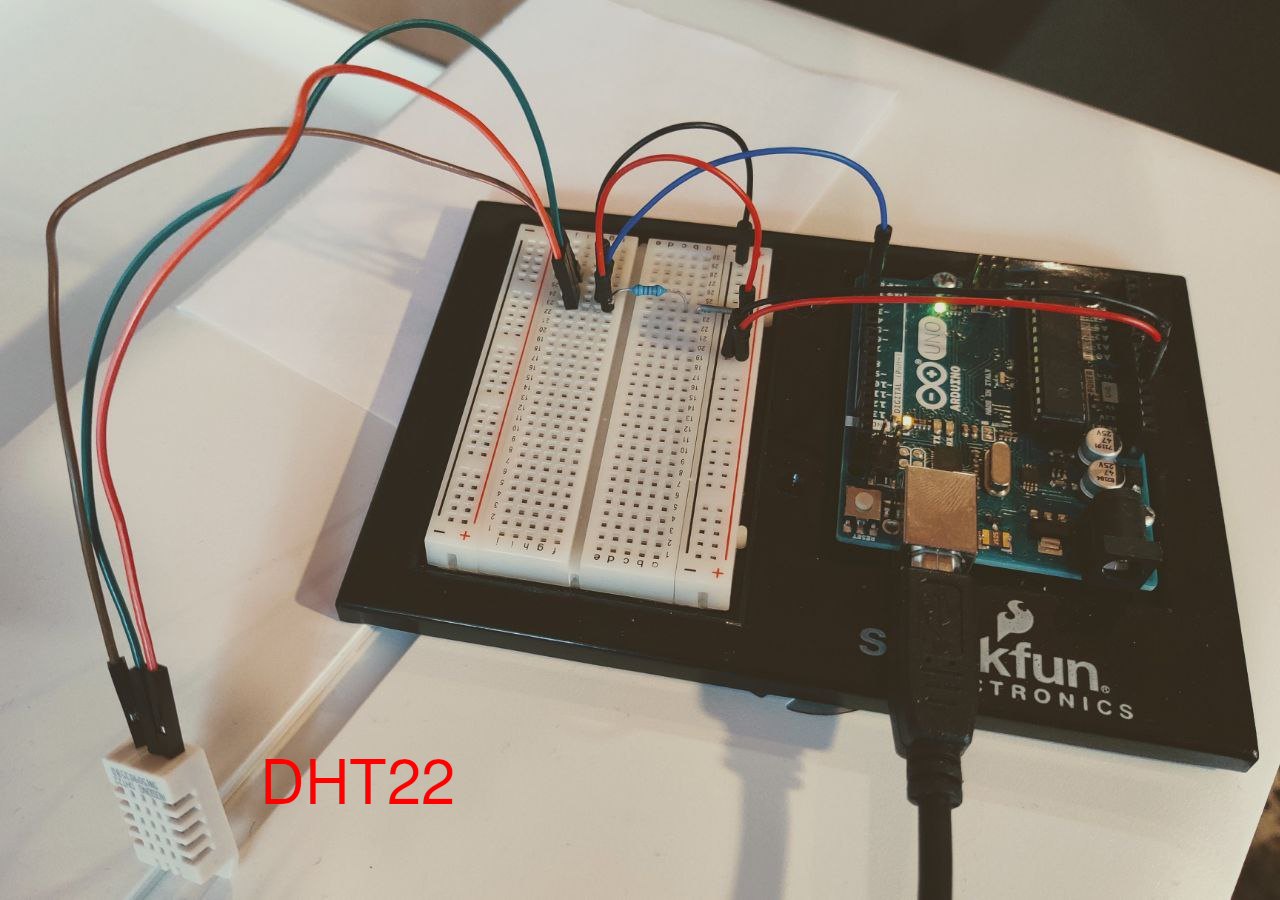
\includegraphics[width=0.4\textwidth]{./pics/journal_paper/DHT22.png}
	\caption{
		Arduino Uno board with attached DHT22 temperature and humidity sensor.
		When it was not cloudy the sun light shined directly on the sensor through the window in the noon causing temperature peaks.
	}
	\label{fig:dht22}
\end{figure}
% Recorded time intervals in hours between beginnings of working days are depicted on the bar plot on Figure~\ref{fig:time_intervals}.
% - \begin{figure}[!htb]
% - 	\centering
% - 	\includegraphics[height=0.3\textheight]{./img/temperature_bars}
% - 	\caption{Time intervals between changes in the temperature signal.
% - % Values are $(21.5, 24.5, 23.7, 23.8, 24.9, 22.9, 25.0, 23.4, 24.0, 24.2, 23.4, 24.5, 25.5)$.
% -   }
% - 	\label{fig:time_intervals}
% - \end{figure}
% The mean and standard deviation values are $\mu=23.95$h $\sigma=1.0$h.
% has a good for $-40$ to $80^{\circ}\text{C}$ temperature readings $\pm0.5^{\circ}\text{C}$ accuracy with no more than 0.5 Hz sampling rate (once every 2 seconds).
Temperature measurements were taken 1 time per 60 seconds using DHT22 temperature and humidity sensor connected to the Arduino board.
Figure~\ref{fig:temperature_signal} illustrates temperature signal.
%To detect changes $CusumMutli$ function (Algorithm~\ref{alg:method_code}) is used.
Figure~\ref{fig:performance_temperature_signal} illustrates results.
% Figure\ref{fig:performance_pccf_temperature_signal} shows Pccf performance for the signal.
\begin{figure}[!htb]
	\centering
	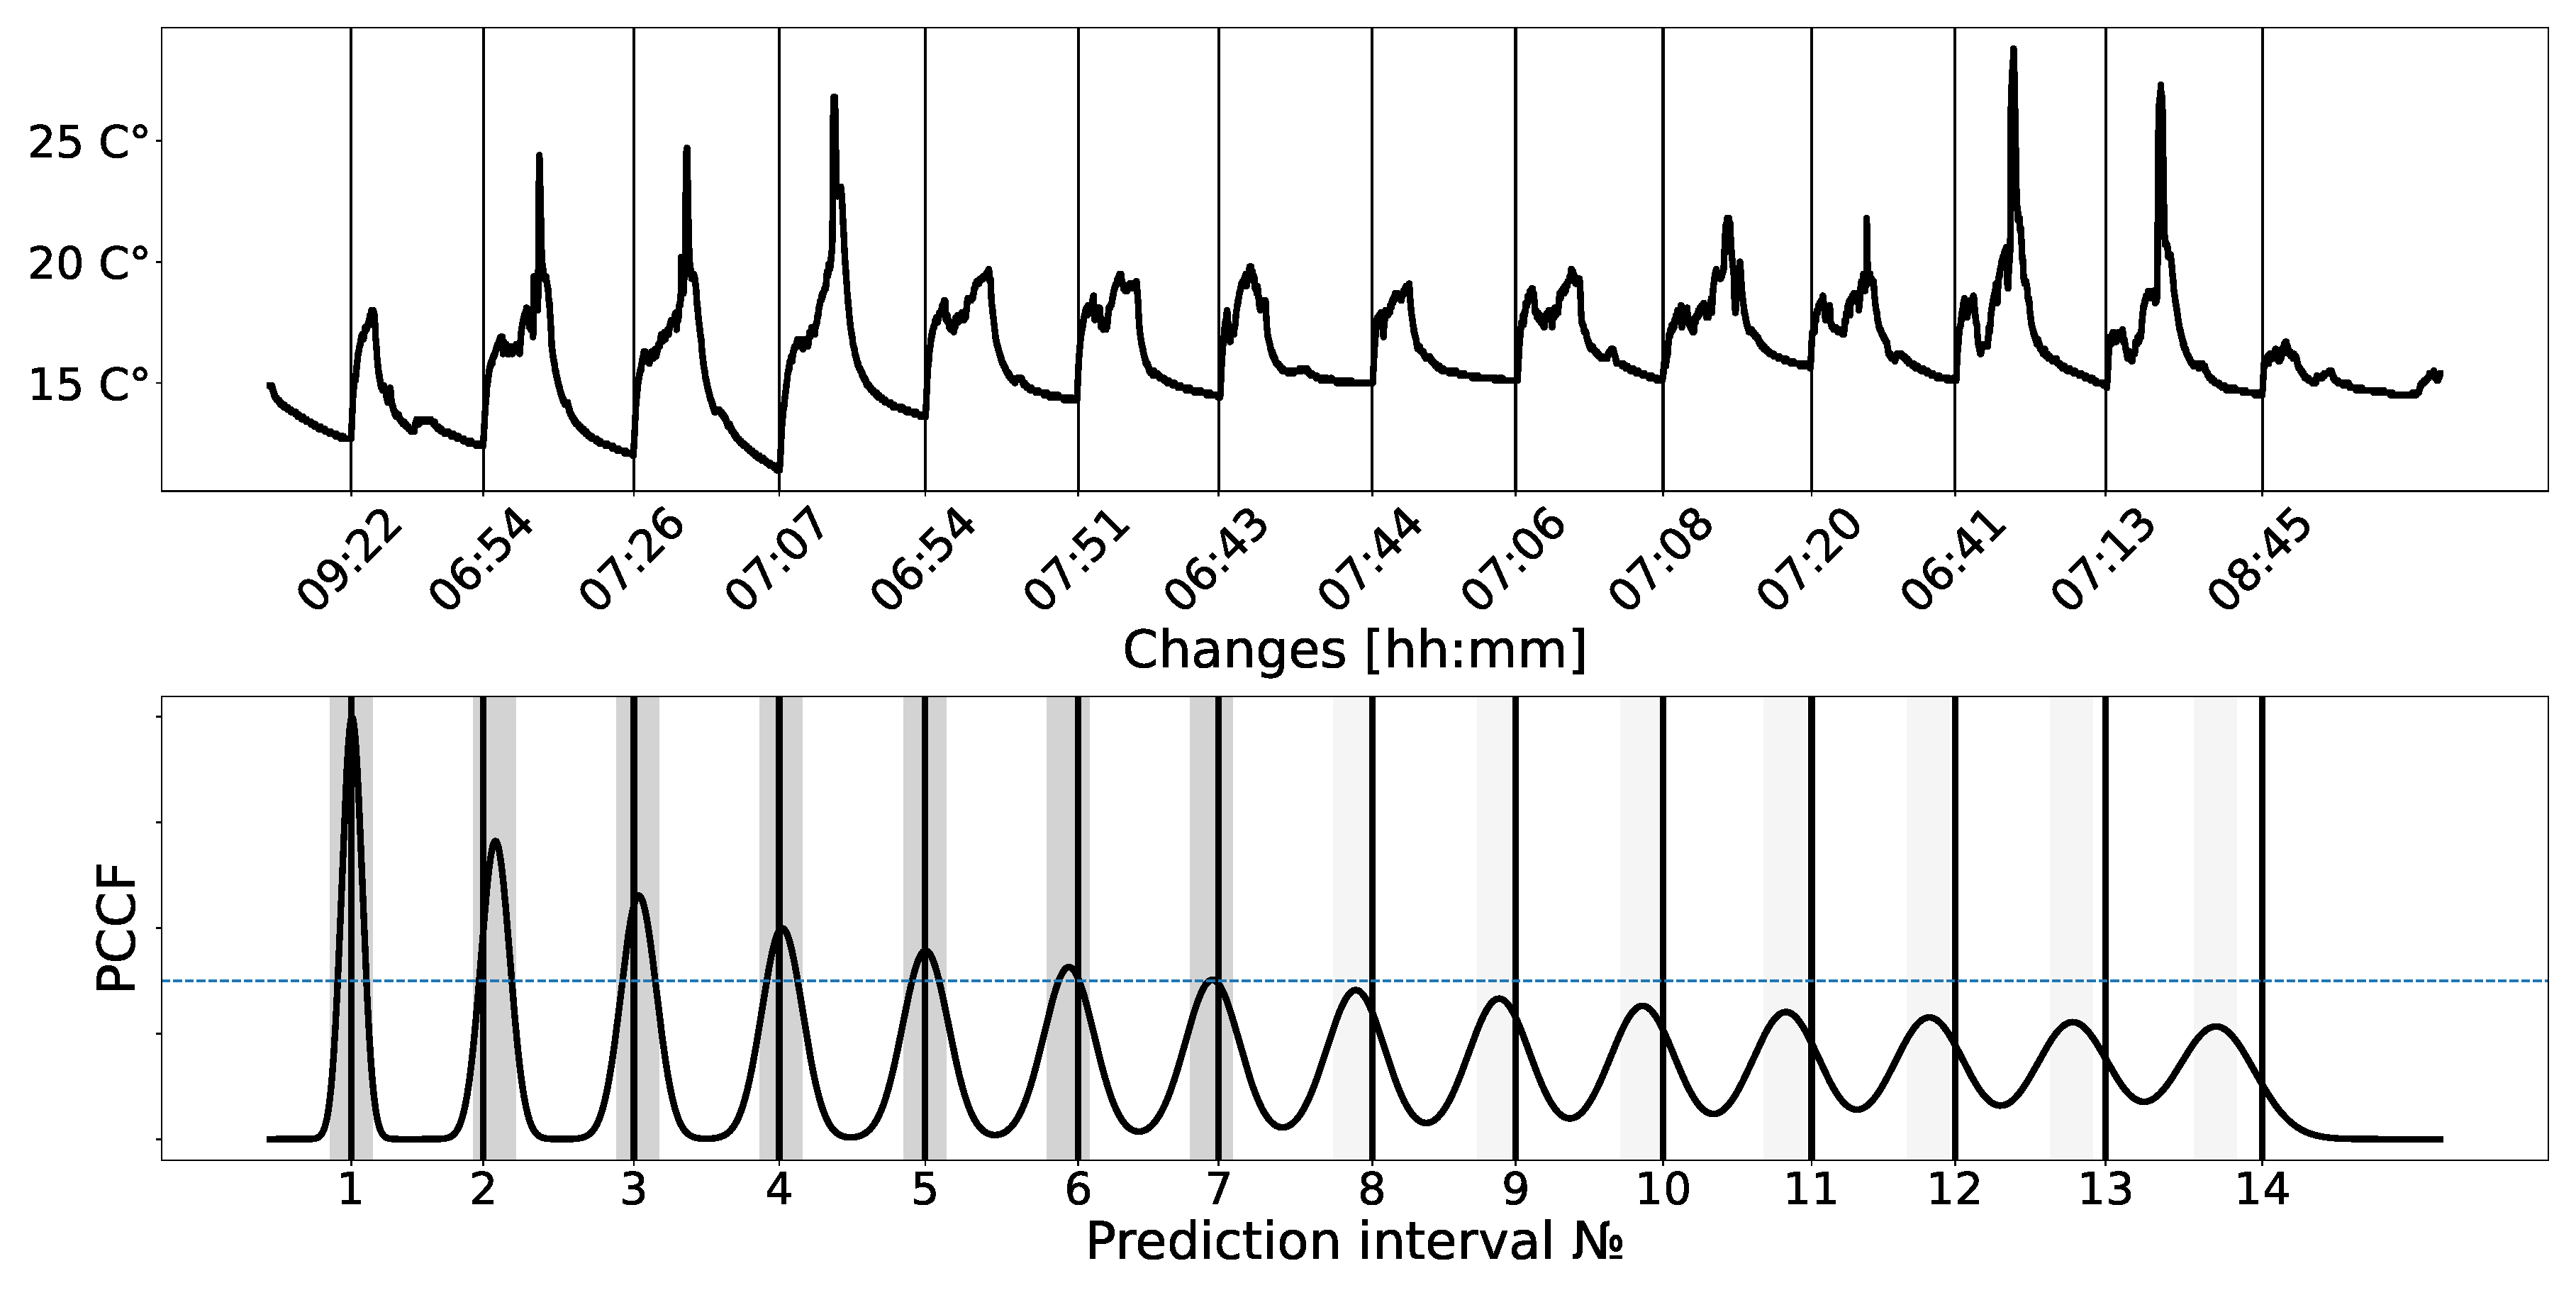
\includegraphics[width=0.9\textwidth]{./pics/journal_paper/temperature_signal}
	\caption{
    Temperature signal and Pccf.
    Changes are depicted by vertical solid lines on both plots.
    Prediction intervals are enumerated and marked by grey vertical regions on the bottom plot. First 7 changes are predicted with a good accuracy, further change points are not within prediction intervals.
  }
	\label{fig:temperature_signal}
\end{figure}
\begin{figure}[!htb]
		\centering
  \begin{tikzpicture}[scale=0.9]
		\draw(0, 0) node{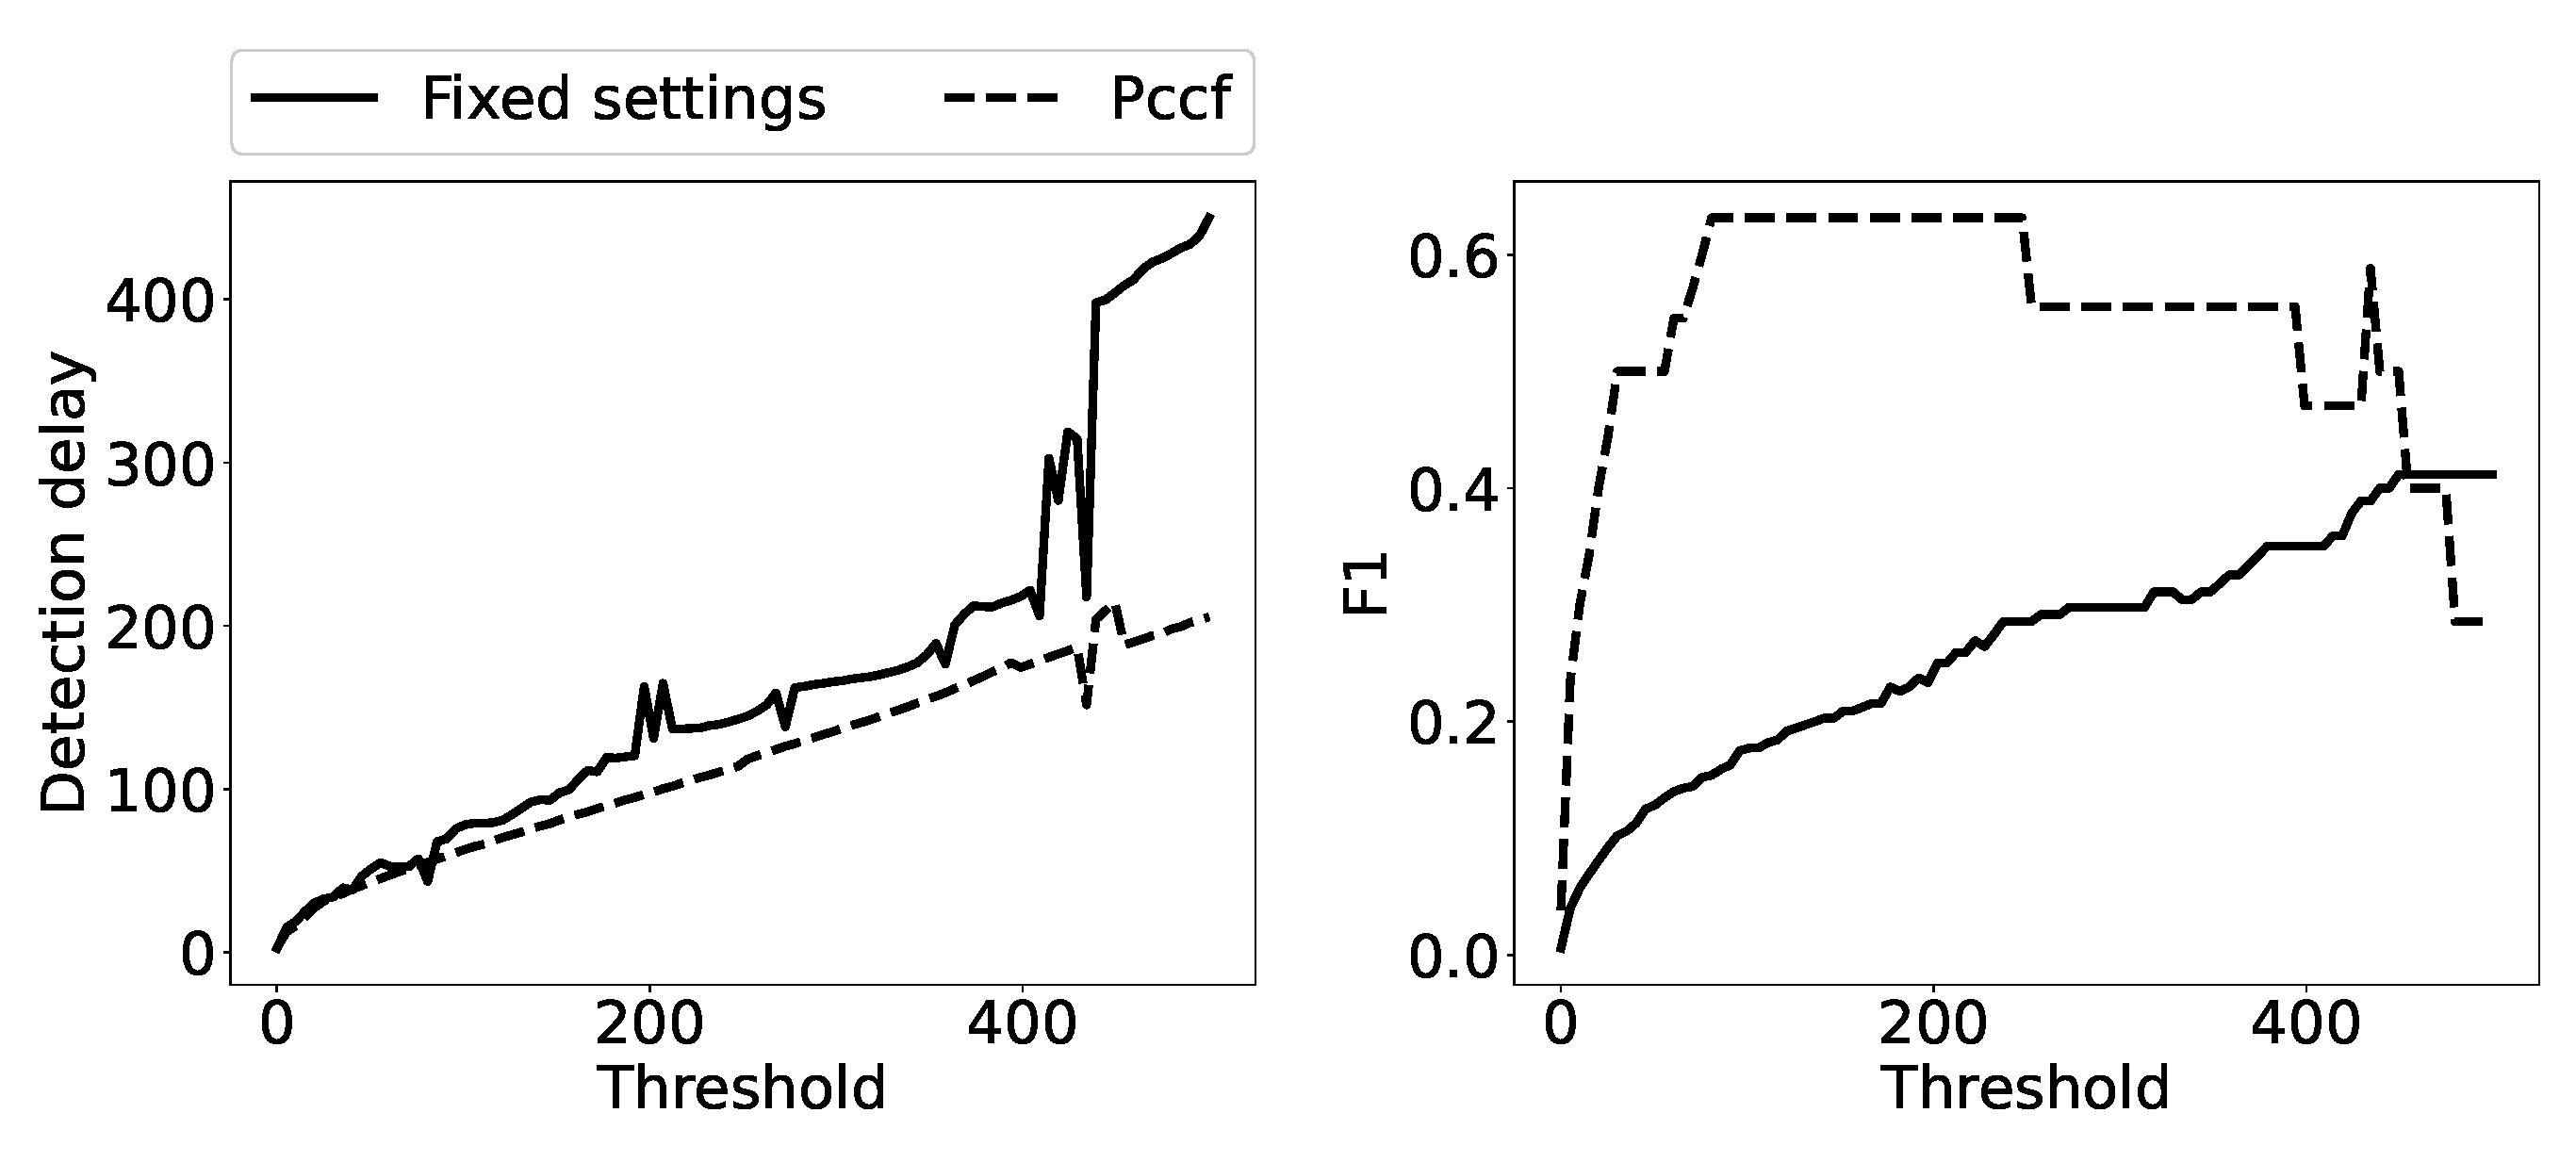
\includegraphics[width=0.8\textwidth]{./pics/journal_paper/performance_temperature_seven}};
		\draw(0, -4.8) node{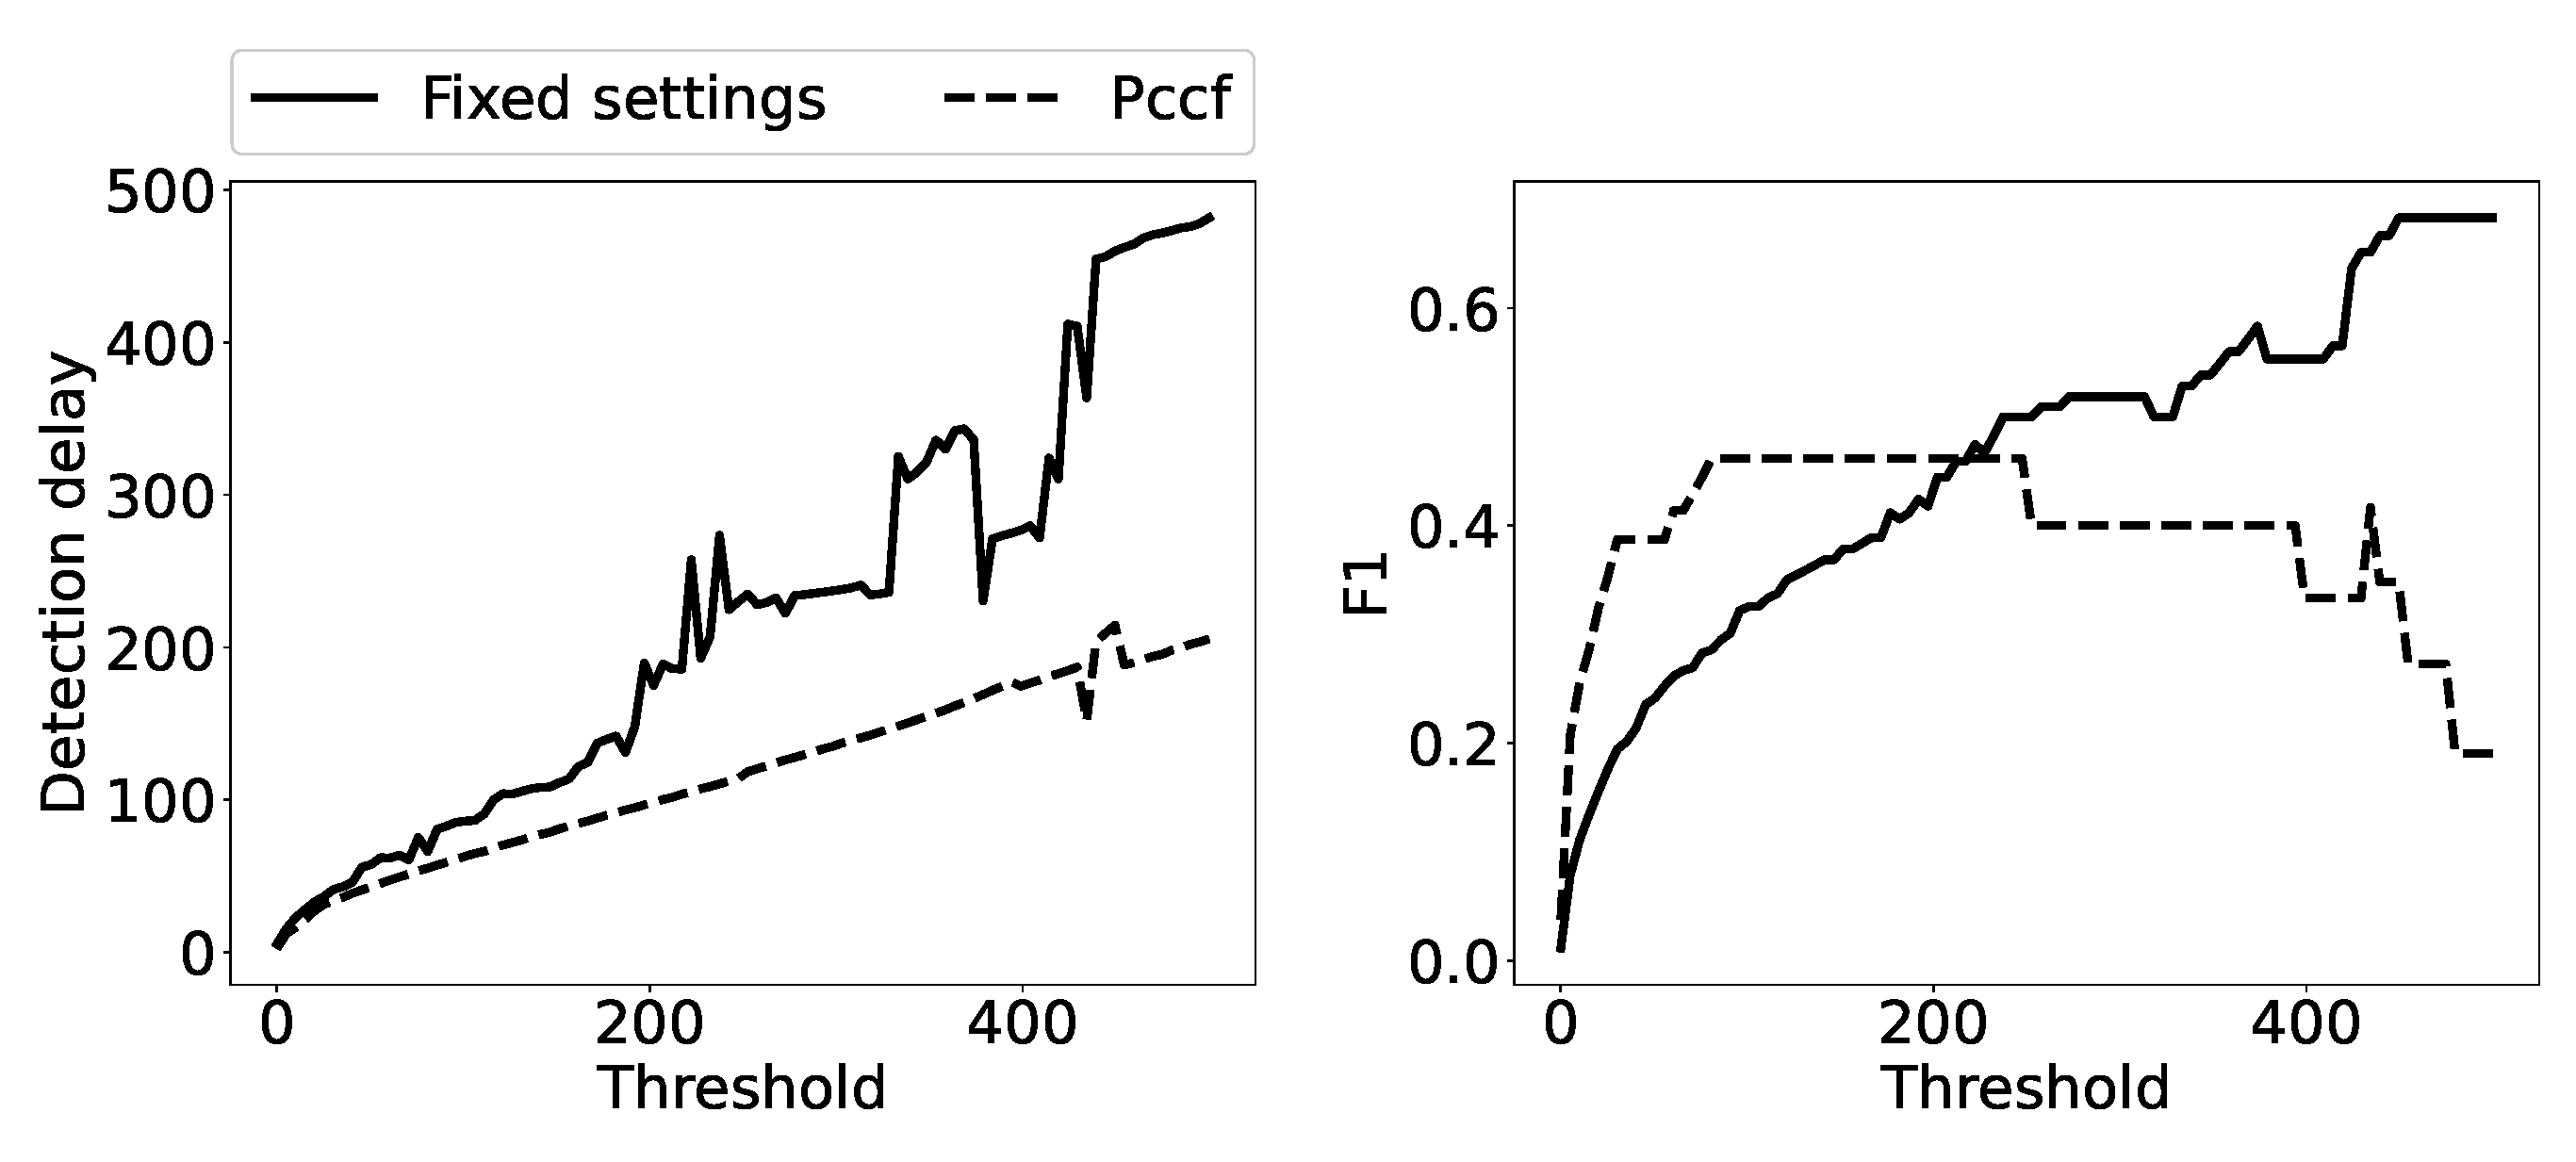
\includegraphics[width=0.8\textwidth]{./pics/journal_paper/performance_temperature}};
		\draw(3, 2.0) node {When predicting 7 changes};
		\draw(3, -2.7) node {When predicting all changes};
	\end{tikzpicture}
  \caption{Detection delay (left side) and $F_1$ score (right side) for the temperature signal when predicting first 7 change points (top) and when trying to predict all changes (bottom). 
  When predicting all changes $F_1$ decreases since Pccf predictions accuracy degrades with the number of change points we are trying to predict. 
  }
	\label{fig:performance_temperature_signal}
\end{figure}

\section{Conclusions}\label{sec:conclusions}
We demonstrated that both detection delay and $F_1$ score can be decreased when using prediction intervals (ROIs) capturing change points locations (Figures~\ref{fig:artificial_signal_perf_results} and ~\ref{fig:performance_temperature_signal}).
Prediction interval width effectively imposes constraints on the maximum detection delay controlled by the detection delay $h$ which, in turn, regulates ARL value (Figure~\ref{fig:arl}, Equation~\ref{eq:arl_approximation}).
If change points are predicted correctly using prediction intervals, then
\begin{enumerate}
    \item At the least, FA rate can be decreased safely just by ignoring all detections outside ROIs
    \item As the next step, detection delay can be decreased too by decreasing detection threshold value $h$ 
    \item When applying lower threshold value within ROI, performance improvement is not guaranteed and is defined by the trade off between outcomes depicted on Figure~\ref{fig:possible_outcomes}.
    % \item If prediction intervals are not correct this leads to additional 
    %\item If static CuSum ARL is within ROI and threshold value $h$ is decreased dynamically then probability of FA is increased (Equation~\ref{eq:arl_approximation}, Figure~\ref{fig:arl}) but due to smaller ROI width in comparison to the whole signal, actual FA rate is still lower than in static case on average.
\end{enumerate}

\subsection{Limitations}
The main limitation of the proposed methodology is a number of additional parameters the user should define.
Specifically, expected time interval between changes should be estimated, number of change points to be predicted, and width of the prediction interval $\text{ROI}_{\text{Width}}$.
Additionally, position of ROI relatively to change point location might play an important role. In this work we considered only symmetrical positioning for simplicity.
%If $\text{ROI}_{\text{Width}}$ is smaller than ARL then detections will happen outside ROI. In that case backtracking mechanism should be used, - this the future work.
%And therefore Cusum output statistic behaves as random walk with the drift before and after changes with unknown trends causing quite bad detection performance.Nevertheless performance was improved significantly in case of predicting 7 change points with the good accuracy.We didn't address options of how prediction intervals are position (symmetrical, or not.)Also, we didn't apply state of the art methods for sequential change detection, but we believe it is not crucial.If $\delta$ is known and therefore ARL approximation can be done than the best strategy would be to backtracking after each detection but in real settings
Another limitation is that incorrect prediction intervals may lead to false alarms being considered as true positives if happened within ROI. IF then new predictions intervals are calculated based on the latest detection it may lead to severely degraded performance. 

\subsection{Future work}
Many public data sets used as a benchmark for concept drift handling algorithms suffer from the common issue of uncertainty about changes~\cite{SouzaRMB20} and lack of the ground truth when change exactly happened. 
In order to have a well defined ground truth data about change points locations we generate time series of observations ourselves.
What potentially might lead to the bias when recording ground truth time moments.
This issue is mitigated by non-stationarity of the temperature signal due to daily fluctuations of the outdoor temperature causing gradual changes with complex pattern.
Additional random abrupt changes were caused by sun light shining on the sensor in case of clear sky. Change points of interest are also not strongly periodical and not all predictable as a whole sequence.
In the future work we plan to include more experiments with real data. 
%Although the signal was generated ourselves - it still contains a lot of uncontrolled factors - samples are clearly not from Gaussian distribution, the pattern is quite complex. The are changes caused not only by the heater, but also changes in the outside temperature, abrupt changes caused by the sun shining directly in the sensor. 

%\newpage
%\appendix
\section{Pseudocode}\label{sec:pseudo_code}
Pseudocode for Cusum detector with and without Pccf.
Full implementation can be found in the GitHub repository~\href{https://github.com/av-maslov/pccf}{https://github.com/av-maslov/pccf}.
\begin{algorithm}
	% class Detector
	\begin{algorithmic}[1]
			%\Function{CusumSingle}{$X$, $h$, $\text{PCCF}$}\Comment{Single changepoint detection}
			%\State n=length($X$)
			%\State stat=zeros(n)
			%\State stat[0]=X[0] - $\mu_0$
			%\For{t $\in$ [1,n]}
			%\State stat[t] = stat[t-1]+X[t]-$\mu_0$
			%\If{(not PCCF) or (PCCF and WithinRoi()) }
			%\If{$|stat[t]| > h$}
			%\State \Return (t, stat) \Comment{Alarm CDE}
			%\EndIf
			%\EndIf
			%\EndFor
			%\State \Return (nan, stat)\Comment{Return missing value for CDE}
			%\EndFunction  
		%\\
		\Function{CusumMutli}{$X$, $h$, $\text{PCCF}$}\Comment{Sequential/multi- changepoint detection}
      \State n = length(Signal)
      \State detections = [ ]
 	  \For{t $\in$ [1,n]}
      %\While{$t <n$}
        \State UpdateMu(Signal[t])
        \State UpdateCusumStatistic()
        \If{PCCF and EnteredRoi()}
          \State NextRoiIndex $\mathrel{{+}{=}} 1$
        \EndIf
        %\Comment{If we don't use Pccf or we use Pccf and we are inside ROI}
        \If{(not PCCF) or (PCCF and WithinRoi()) }
        \If{$|stat[t]| > h$}
          \State detections.append(t) \Comment{Collect CDEs}
          \State ResetDetector()
        \EndIf
        \EndIf
        %\State t $\mathrel{{+}{=}} 1$
      %\EndWhile
      \EndFor
      \If{len(detections) == 0} \Comment{In case of detecting single change point}
        \State delay = NaN \Comment{Return detection delay NaN if no detection is alarmed}
      \EndIf
      \State \Return detections 
		\EndFunction
		\\
		\Function{UpdateMu}{}\Comment{Running mean value after each CDE}
      \State $\mu_{t}=\frac{k-1}{k} \mu_{t-1} + \frac{x}{k}  $
		\EndFunction
		\\
		\Function{UpdateCusumStatistic}{}\Comment{Update CUSUM statistic}
      \State $\delta = x_t - \mu_t$
      \State $stat[0] = \delta$
      \State $stat[t] = stat[t-1] + \delta \: \forall \: t >0$
		\EndFunction
		\\
		\Function{ResetDetector}{}\Comment{Re-initialize detector after each CDE}
      \State $\mu_t=0$
      \State k=1
      \State $stat[t]=x_t$
		\EndFunction
	\end{algorithmic}
	\caption{Cusum for single and multiple change points detection.}\label{alg:method_code}
\end{algorithm}


% \begin{abstract}
% % \PACS{PACS code1 \and PACS code2 \and more}
% % \subclass{MSC code1 \and MSC code2 \and more}
% \end{abstract}
%
% % For two-column wide figures use
% \begin{figure*}
% % Use the relevant command to insert your figure file.
% % For example, with the graphicx package use
%   \includegraphics[width=0.75\textwidth]{example.eps}
% % figure caption is below the figure
% \caption{Please write your figure caption here}
% \label{fig:2}       % Give a unique label
% \end{figure*}
% %
% % For tables use
% \begin{table}
% % table caption is above the table
% \caption{Please write your table caption here}
% \label{tab:1}       % Give a unique label
% % For LaTeX tables use
% \begin{tabular}{lll}
% \hline\noalign{\smallskip}
% first & second & third  \\
% \noalign{\smallskip}\hline\noalign{\smallskip}
% number & number & number \\
% number & number & number \\
% \noalign{\smallskip}\hline
% \end{tabular}
% \end{table}
%
%\begin{acknowledgements}
%If you'd like to thank anyone, place your comments here
%and remove the percent signs.
%\end{acknowledgements}
%
% Authors must disclose all relationships or interests that
% could have direct or potential influence or impart bias on
% the work:
%
% \section*{Conflict of interest}
%
% The authors declare that they have no conflict of interest.
%
% BibTeX users please use one of
%\bibliographystyle{spbasic}      % basic style, author-year citations

